%%%%%%%%%%%%%%%%%%%%%%%%%%%%%%%%%%%%%%%%%%%%%%%%%%%%%%%%%%
%
% Doctoral Thesis Template @ The University of Manchester
% LaTeX Chapter Template
% Version 1 (23/07/2020)
% Joe Crone
%
% This template is based on:
% The University of Manchester, Presentation of Thesis Policy
% Research Office Graduate Education Team
% June 2017
% http://www.regulations.manchester.ac.uk/pgr-presentation-theses/
%
%%%%%%%%%%%%%%%%%%%%%%%%%%%%%%%%%%%%%%%%%%%%%%%%%%%%%%%%%%
\documentclass[../main.tex]{subfiles}
\begin{document}

% Title
%--------------------------------------------------------
\chapter{Photon Production by Inverse Compton Scattering}
\label{Photon_Production_by_Inverse_Compton_Scattering} % to reference use \ref{ChapterTemplate}

\section{Electron - Photon Interactions}
\label{sec:electron_photon_interactions}

While scattering interactions, specifically inverse Compton scattering interactions, are possible from all particles, the work presented here is only concerned with electron--photon interactions, the most commonly utilised form of inverse Compton scattering.  Electron--photon interactions are advantageous over other particle--photon interactions due to their low rest mass $m_{e}c^{2}$, resulting in a typically large Lorentz factor, which allows for the production of high energy photons as the scattered photon energy $E_{\gamma}$ of an ICS interaction is proportional to the Lorentz factor (Eq.~\ref{eq:Lorentz_factor}) squared ($E_{\gamma}\propto\gamma^{2}$) i.e a double Doppler shift occurs. Within this chapter, we briefly review electron--photon interactions in general, with a focus on inverse Compton scattering, present the relevant laser physics, then extend this work to ICS photon--electron interactions on a collective basis (electron bunch--photon pulse interactions) and define several parameters to characterise the performance of radiation generation based on ICS.   

The simplest form of electron--photon interaction is Thomson scattering \cite{thomson1904xxxiv}, where an incident photon accelerates a charged particle and the charged particle subsequently emits a photon of identical energy, we assume the collision is elastic and therefore $p_{1} = p_{2}$ -- where $p_{1}$ is the incident electron energy and $p_{2}$ is the final electron energy -- such that the recoil of the electron is negligible. The criterion for the photon--electron interaction to be modelled by Thomson scattering is when the energy of the photon $E_{L}=\hbar\omega$ is much smaller than the rest mass of the electron ($m_{e}c^{2}\gg E_{L}$). Thomson's electron--photon interaction model was furthered by Compton \cite{compton1923quantum}, where the inelastic scattering case ($p_{1} \neq p_{2}$) -- named Compton scattering -- is modelled; the electron recoils and the photon is scattered with a different wavelength to the wavelength of the incident photon . Within this thesis, we are concerned with inverse Compton scattering -- the process of scattering a photon from a relativistically-moving electron in which the scattered photon energy is double Doppler shifted, and the scattered photon parasitically gains energy from the recoiling electron. Specifically, we are interested in inverse Compton scattering sources where an incident bunch of electrons is interacted with an incident photon pulse, as detailed in Section~\ref{sec:lasers_fabry_perot}. 

Photon--electron interactions can be represented with complete generality by using the two quantum electrodynamic leading order Feynman diagrams as shown in Fig.~\ref{fig:ICS_Feynman_diagrams}. 
\begin{figure}[!h]
\centering
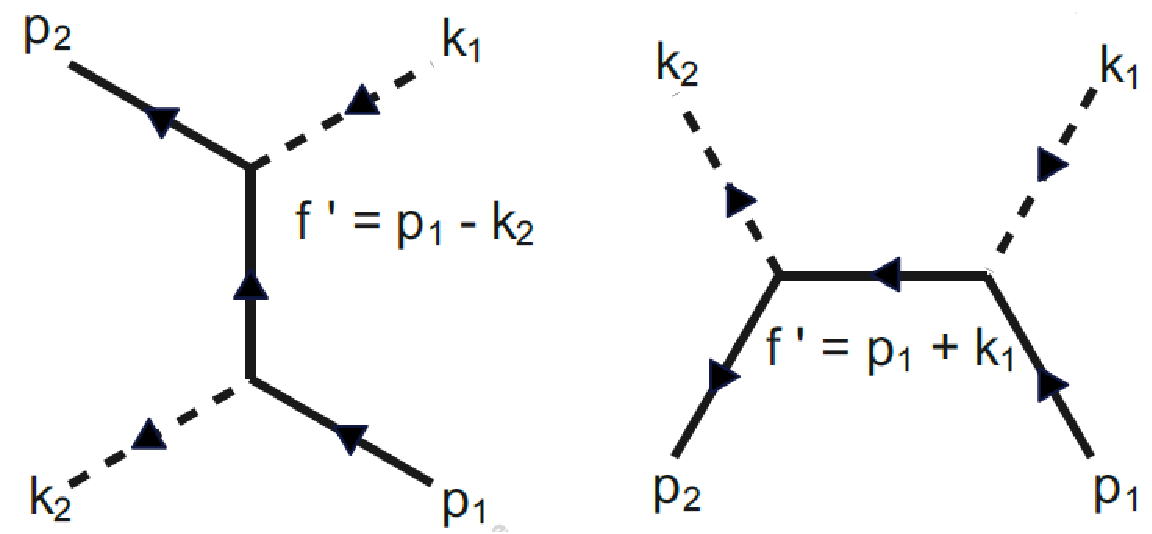
\includegraphics[width=0.65\textwidth]{Figures/Photon_Production_by_Inverse_Compton_Scattering/ICS_feynman_fixed.pdf}
\caption{Two tree-level Feynman diagrams of photon (dashed)--electron (solid) interactions, which contribute to the matrix element of the (inverse) Compton scattering process \cite{berestetskii1982quantum}. Left: The scattered photon $k_{2}$ is emitted with the annihilation of the incident electron $p_{1}$, and the incident photon $k_{1}$ is absorbed with the production of the recoiling electron $p_{2}$. Right: The incident photon $k_{1}$ and electron $p_{1}$ are absorbed, and the scattered photon $k_{2}$ is emitted with the recoiling electron $p_{2}$.}
\label{fig:ICS_Feynman_diagrams}
\end{figure}
The general form of the electron--photon interactions can be specified by
\begin{equation}
p_{1} + k_{1} = p_{2} + k_{2},
\label{eq:ICS_process}
\end{equation}
where $p_{1}$ is the four-momenta of the incident electron, $k_{1}$ is the four-momenta of the incident photon, $p_{2}$ is the four-momenta of the recoiling electron, and $k_{2}$ is the four-momenta of the scattered photon. The geometry of the inverse Compton scattering interaction in a 2D plane is shown in Fig.~\ref{fig:scattered_photon_kinematics}.

\begin{figure}[!h]
\centering
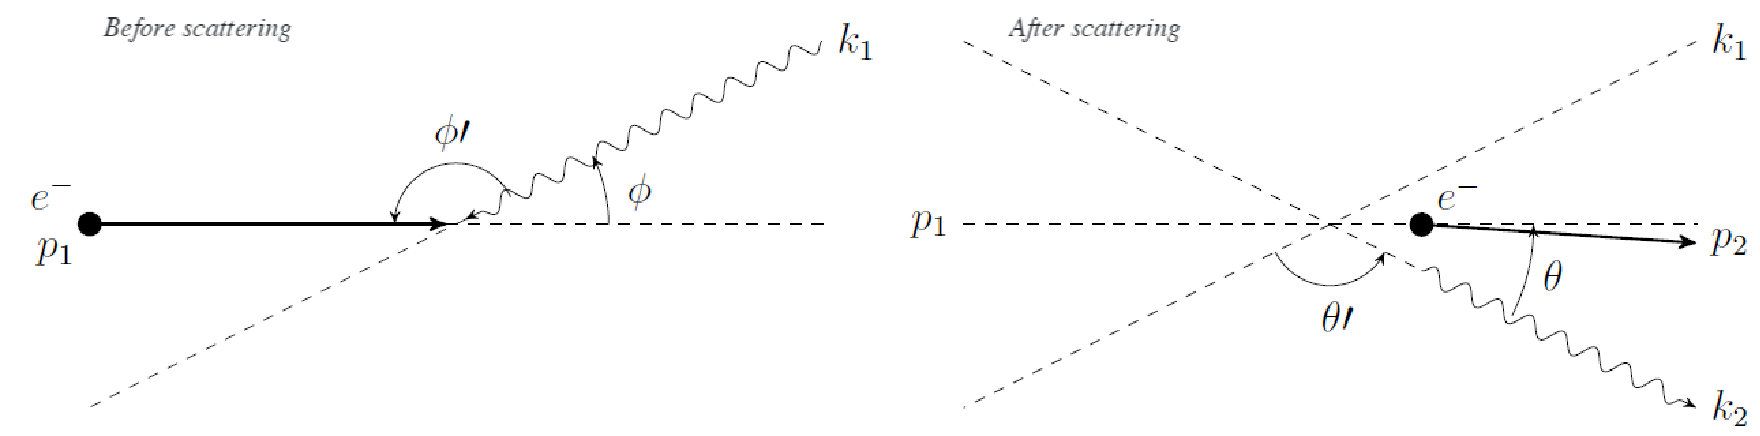
\includegraphics[width=\textwidth]{Figures/Photon_Production_by_Inverse_Compton_Scattering/scatteringkinematicsdiagram.pdf}
\caption{Geometry of the inverse Compton scattering event at the interaction point. The interaction geometry follows the geometry prescribed by Sun et al \cite{sun2009energy}. Here $\theta$ is the scattering angle of the photon, with $\phi' = \pi -\phi$, the angle between the incident electron and incident photon, where $\phi$ is the crossing angle of the electron and photon and $\theta' = \pi - \theta - \phi$ the angle between the incident and scattered photon. Left: Before interaction. Right: After interaction.}
\label{fig:scattered_photon_kinematics}
\end{figure}

Motivated by the geometry of the inverse Compton scattering process, as shown in Fig.~\ref{fig:scattered_photon_kinematics}, the initial photon $p_{1}$ and electron $k_{1}$ four-momenta can be expressed by
\begin{align}
p_{1} &= \gamma m_{e}\left(c,\boldsymbol{v_{i}}\right),
\label{eq:initial_four_vectors} \\
k_{1} &= \frac{E_{L}}{c}\left(1,\hat{n}_{i}\right), 
\end{align}
where $E_{L}$ is the energy of the incident photon, $\hat{n}_{i}$ is the unit displacement three-vector of the incident photon, $\gamma$ is the Lorentz factor, $m_{e}$ is the mass of the electron, $c$ the speed of light in a vacuum and $\boldsymbol{v_{i}}$ is the velocity three-vector of the incident electron with magnitude $v_{i}$. Similarly, we can present the final electron and scattered photon states with four-momenta 
\begin{align}
p_{2} &= \gamma' m_{e}\left(c,\boldsymbol{v_{f}}\right), \\
k_{2} &= \frac{E_{\gamma}}{c}\left(1,\hat{n}_{f}\right), 
\label{eq:final_four_vectors} 
\end{align}
where $E_{\gamma}$ is the scattered photon energy, $\hat{n}_{f}$ is the unit displacement three-vector of the scattered photon, $\gamma'$ is the Lorentz factor of the recoiling electron and $\boldsymbol{v_{f}}$ is the velocity three-vector of the recoiling electron with magnitude $v_{f}$.

Using the four-momenta definitions (Eq.~\ref{eq:initial_four_vectors}-\ref{eq:final_four_vectors}), a  series of kinematic invariants (Mandelstam variables \cite{mandelstam1958determination}) can be determined for the photon-electron scattering process \cite{berestetskii1982quantum}
\begin{align}
s &= \left(p_{1}+k_{1}\right)^{2} = \left(p_{2}+k_{2}\right)^{2},
\label{eq:s_Mandelstam} \\
t &= \left(p_{1}-p_{2}\right)^{2} = \left(k_{2}-k_{1}\right)^{2},
\label{eq:t_Mandelstam} \\
u &= \left(p_{1}-k_{2}\right)^{2} = \left(p_{2}-k_{1}\right)^{2}.
\label{eq:u_Mandelstam}
\end{align}
where $t$ desribes the momentum transfer of the process, $s$ is the centre of mass energy squared and $u$ has more tenuous physical meaning, describing the cross-channel of the interaction \cite{berestetskii1982quantum}. The kinematic invariants can be used to form more convenient Lorentz invariants
\begin{align}
X &= \frac{s-\left(m_{e}c\right)^{2}}{\left(m_{e}c\right)^{2}},
\label{eq:X_Mandelstam} \\
Y &= \frac{\left(m_{e}c\right)^{2}-u}{\left(m_{e}c\right)^{2}},
\label{eq:Y_Mandelstam}
\end{align}
which, when transformed into the geometry as shown in Fig.~\ref{fig:scattered_photon_kinematics}, can be re-wrote as
\begin{align}
X &= \frac{2\gamma E_{L}\left(1+\beta\cos\phi\right)}{m_{e}c^{2}},
\label{eq:X_geometry} \\
Y &= \frac{2\gamma E_{\gamma}\left(1-\beta\cos\theta\right)}{m_{e}c^{2}},
\label{eq:Y_geometry}
\end{align}
where $\beta = v/c$ is the Lorentz speed factor.

Taking the head-on interaction case ($\phi = 0$) and assuming the incident electron is ultra-relativistic ($\beta \rightarrow 1$), the $X$ invariant simplifies to 
\begin{equation}
X = \frac{4\gamma E_{L}}{m_{e}c^{2}}.
\label{eq:X_headon}
\end{equation}
The Lorentz invariant $X$ can also be termed the recoil parameter, which denotes the magnitude of the recoil of the incident electron. For the case $X \ll 1$, the recoil is small and inverse Compton scattering reduces to Thomson scattering, the interaction becomes elastic. To illustrate, assuming a head-on interaction ($\phi=0$) with a near-infrared laser (Nd:YAG, $\lambda = 1064$~\si{\nano\meter}, see Section~\ref{sec:lasers_fabry_perot}), a 1\% recoil effect ($X = 0.01$) requires an electron kinetic energy of $E_{e} = 558$~\si{\mega\electronvolt}, via re-arrangement of (Eq.~\ref{eq:X_headon}). For a visible green wavelength ($\lambda = 532$~\si{\nano\meter}), a electron kinetic energy $E_{e} = 279$~\si{\mega\electronvolt} is required. Therefore, as the sources designed in this thesis typically use near-infrared incident photons (as explained in Section~\ref{sec:lasers_fabry_perot}), recoil effects are expected to be non-negligible only in designs for $\gamma$-ray ICS sources (where the electron beam energy is 100's~\si{\mega\electronvolt}).   

\section{Lasers and Fabry--Perot Optical Re-circulation Cavities}
\label{sec:lasers_fabry_perot}

Inverse Compton scattering sources, which use the inverse Compton scattering process to produce beams of Doppler-shifter scattered radiation, require a source of incident photons. Ideally the incident photon beam will be monochromatic, have a high power and be of small physical dimensions upon interaction (as explained in future sections) to produce a scattered photon beam with identical characteristics. The incident photon beam criteria is satisfied for two photon sources: accelerator produced radiation, such as synchrotron radiation and free electron lasers, and lasers. Within this thesis only lasers are considered as incident photon sources for ICS sources, as accelerator produced radiation can only be attained on particle accelerators already utilised as radiation sources.

ICS sources can be designed using two approaches we term `single shot' and `re-circulated pulse', which relate to design of the optical system -- A schematic of each is shown in Fig.~\ref{fig:single_shot_4mirror}. In `single shot' ICS sources each incident photon pulse is used once; typically a high peak power laser pulse, with up to Joule-scale laser pulse energies and pulse durations in the range 1~\si{\pico\second}--10~\si{\femto\second}, is interacted with an electron bunch to scatter photons. The limitation on the interaction rate (repetition rate) of the source is due to the repetition rate of the laser pulse, which is often limited to the \si{\hertz} to \si{\kilo\hertz} scale. However, re-circulated accelerators have 10--100~\si{\mega\hertz} bunch repetition rates and linear accelerators typically operate with bunch repetition rates on the \si{\kilo\hertz}-scale, so the `single shot' approach is most advantageous for linear accelerators. As detailed in Section~\ref{sec:nonlinear_ICS}, high energy laser pulses can cause non-linear ICS interactions, which may be beneficial for ICS source development and is most achievable with this configuration. 

\begin{figure}[!h]
\centering
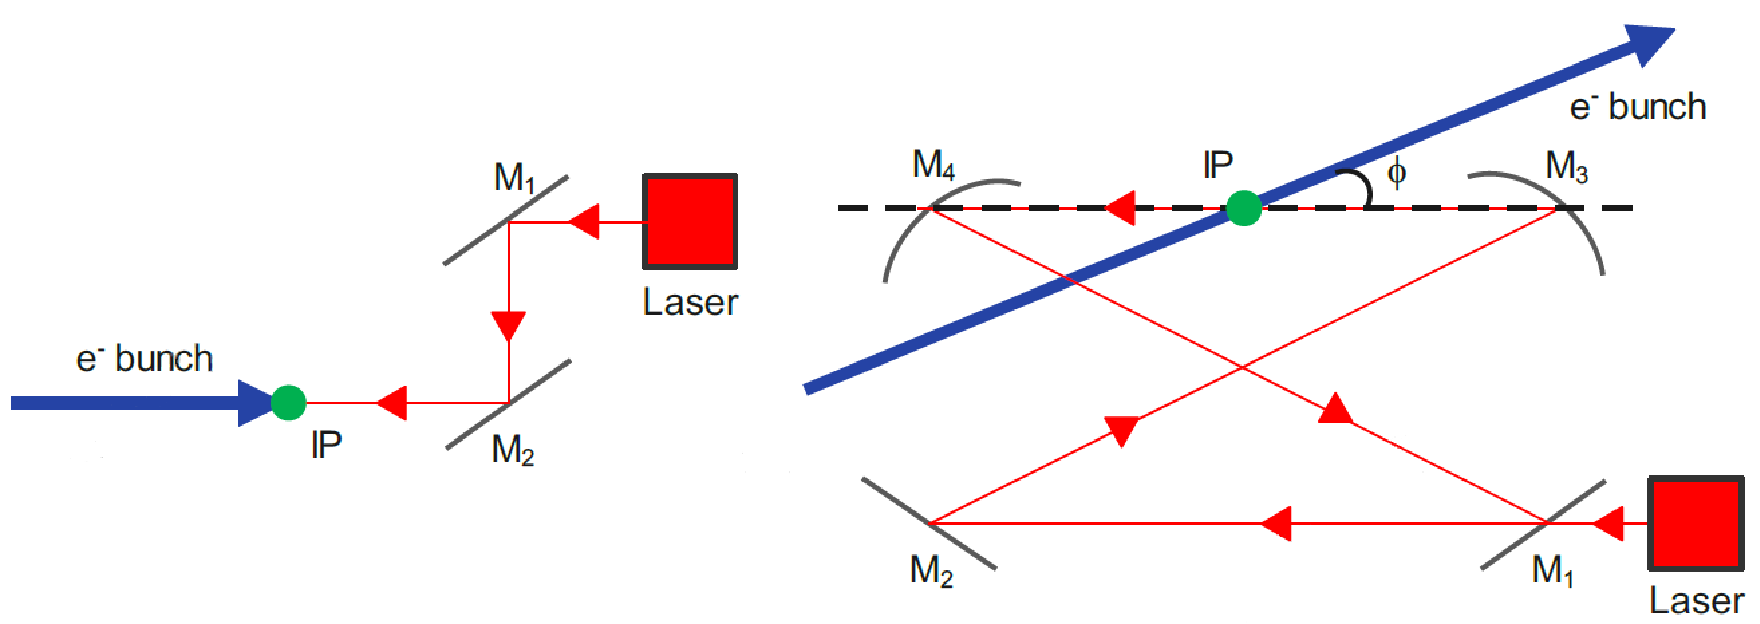
\includegraphics[width=\textwidth]{Figures/Photon_Production_by_Inverse_Compton_Scattering/single_shot_4_mirror.pdf}
\caption{Possible interaction configurations for ICS sources. Left: `Single shot' ICS source, where a laser pulse (red) is generated and interacted at the interaction point (green) in a head-on ($\phi=0$) geometry with the electron bunch (blue). Mirrors (grey) are used to transport the laser pulse to the IP. Right: `Re-circulated pulse' ICS source, where a laser pulse (red) is interacted with the electron bunch (blue) at the IP (green). The laser pulse is re-circulated by the mirrors (grey) of the optical cavity and re-interacted with the next recirculated electron bunch.}
\label{fig:single_shot_4mirror}
\end{figure}

Alternatively, the `re-circulated pulse' approach utilises a re-circulated laser pulse where a series of mirrors are used to reflect the laser pulse (or laser pulses) to the interaction point many times. Re-circulation of the laser pulse is achieved by Fabry-Perot optical cavities, detailed in Section~\ref{sec:fabry_perot_optical_cavities}. Re-circulation of the incident photon pulse enables a higher photon pulse repetition rate of around 10--100's~\si{\mega\hertz}, increasing the interaction frequency of the ICS source, and therefore increasing the number of potential photon scattering events. A higher repetition rate of the laser pulse means this approach is more useful for re-circulated accelerators such as storage rings and ERLs. However, re-circulation of the laser pulse places limitations upon the laser pulse energy that may be recirculated -- Joule-scale pulse re-circulation has not been demonstrated -- which is further explored in Section~\ref{sec:fabry_perot_optical_cavities}. Non-linear ICS sources may also be excluded from the `re-circulated pulse' approach as the reduced pulse energies in re-circulated optical cavities may not achieve the intensity required for non-linear ICS.     

\subsection{Lasers for Inverse Compton Scattering Sources}
\label{sec:ICS_lasers}

Lasers providing the incident photon pulse for an ICS source are selected due to wavelength (incident photon energy), the pulse duration, the compatibility with optical mirror technologies -- high reflectivity optical mirror coatings are only available in certain wavelength regimes -- and the spectral bandwidth of the radiation. Certain lasers do not produce photons in continuous wave mode but are pulsed; continuous wave lasers have a higher repetition frequency and therefore are those considered for `re-circulated' pulse operation. Many lasers are applicable to ICS sources and this discussion is not comprehensive, but to illustrate the above criteria we consider: CO$_{2}$ ($\lambda=10.6$~\si{\micro\meter}) \cite{ovodenko2016high}, Ti:Sa ($\lambda=800$~\si{\nano\meter}) \cite{thorlabs2021tisa}, Nd:YAG ($\lambda=1064$~\si{\nano\meter}) \cite{thorlabs2021ndyag450,thorlabs2021ndyag200} and a frequency doubled Nd:YAG laser ($\lambda=532~\si{\nano\meter}$) \cite{chauchat2010instrumentation}.

A CO$_{2}$ laser has the longest wavelength ($\lambda=10.6~\si{\micro\meter}$), resulting in the least energetic photons ($E_{L}=0.117$~\si{\electronvolt}), which by inspection of (Eq.~\ref{eq:scattered_photon_energy}) means higher energy electrons are required for x-ray and $\gamma$-ray production in comparison to other lasers. However, for invariant laser pulse energy more photons are present in the pulse -- for a 100~\si{\micro\joule} laser pulse energy a CO$_{2}$ laser pulse contains $5.33\times 10^{15}$ photons, whereas a $\lambda=1$~\si{\micro\meter} laser pulse contains $5.03\times 10^{14}$ photons -- which means more scattered photons can be generated from the same pulse energy. CO$_{2}$ lasers are pulsed with pulse repetition frequencies of around 15~\si{\kilo\hertz} \cite{pogorelsky2020converting}, so have limited applicability in re-circulated ICS sources. Optical mirrors are available commercially within this range, with reflection coefficients of $R>0.99$ and damage thresholds of 10~\si{\kilo\watt}/\si{\centi\meter}$^{2}$ \cite{thorlabs2021co2optics}. The pulse duration of CO$_{2}$ lasers is long $\sim 100$'s~\si{\pico\second}, but is modulated into sub-pulses which can be of around 5~\si{\pico\second} \cite{pogorelsky2020converting, ovodenko2016high} limiting the duration of produced radiation. The \textit{rms} spectral bandwidth of the CO$_{2}$ laser pulse is narrow ($\Delta E_{L}/E_{L} = 4.95\times 10^{-4}$) \cite{tochitsky2016prospects}, which would allow for the production of narrowband radiation.

Titanium-Sapphire (Ti:Sa) laser systems have a wavelength of $\lambda=800$~\si{\nano\meter}, in the near-infrared regime with photon energies of $E_{L} =1.55$~\si{\electronvolt}, allowing easier access to x-ray and $\gamma$-ray scattered photon energies (Eq.~\ref{eq:scattered_photon_energy}) than CO$_{2}$ lasers. Chirped pulse amplification (CPA) \cite{strickland1985compression} is frequently used with Ti:Sa lasers to obtain high pulse powers on the Joule-scale, for example the COHERENT laser at the ALICE ICS demonstration \cite{priebe2008inverse}, which has a pulse energy of 0.86~\si{\joule} at a repetition frequency of 10~\si{\hertz}. High pulse energies increase the number of photons scattered per electron bunch--laser pulse interaction however, with a repetition frequency of 10~\si{\hertz}, the average laser power is limited to 8.6~\si{\watt}. The repetition rate is not ideal for interaction with electron bunches re-circulated at 100's~\si{\mega\hertz}. Bunch durations of CPA Ti:Sa lasers are very short, for example the COHERENT system has a bunch duration of 35~\si{\femto\second} FWHM,  allowing generation of short duration scattered photon pulses useful in some experiments. High reflection co-efficient mirrors $R>0.99$ are available commercially for Ti:Sa lasers \cite{thorlabs2021tisaoptics}. However, Ti:Sa lasers typically have very large spectral bandwidth, for example $\Delta E_{L}/E_{L} = 0.0442$ for the COHERENT laser system \cite{priebe2008inverse} and $\Delta E_{L}/E_{L}=0.0884$ for a commercial Ti:Sa system \cite{thorlabs2021tisa}. A large spectral bandwidth limits the bandwidth of the scattered photons and therefore a Ti:Sa laser is not ideal for narrowband photon generation.

An Nd:YAG laser has a near-infrared wavelength of $\lambda=1064$~\si{\nano\meter}, corresponding to an incident photon energy of $E_{L}=1.17$~\si{\electronvolt}, which means high energy photons, such as $\gamma$-rays, are more achievable than with a CO$_{2}$ laser systems. Because Nd:YAG lasers can be operated in continuous wave mode they are applicable to `re-circulated pulse' ICS sources. \textit{Rms} pulse durations of Nd:YAG lasers are typically 5--20~\si{\pico\second} \cite{pogorelsky2020converting,akagi2016narrow}, allowing for for production of short duration (\si{\pico\second}-scale) radiation. Very high reflection co-efficient mirrors (R>0.995) are available commercially for Nd:YAG lasers, meaning the incident photon pulse can be transported with low loss and the mirrors have a high damage threshold of 20~\si{\kilo\watt}/\si{\centi\meter}$^{2}$ \cite{thorlabs2021ndyagoptics} -- ideal for high average power re-circulation. Nd:YAG lasers have a very narrow \textit{rms} spectral bandwidth, useful for design of a narrow bandwidth ICS source. For example, a commercial laser system \cite{thorlabs2021ndyag200} has a narrow \textit{rms} spectral bandwidth of $\Delta E_{L}/E_{L} = 4.70\times 10^{-4}$. 

Many lasers may be frequency doubled (second harmonic generation) \cite{franken1961generation} where an incident photon pulse passing through a non-linear crystal material can generate a new pulse with half the incident wavelength. An Nd:YAG laser may be frequency doubled to reduce the wavelength from $\lambda=1064$~\si{\nano\meter} to $\lambda=532$~\si{\nano\meter} \cite{kozlovsky1988efficient}, which has an incident photon energy of $E_{L}=2.34$~\si{\electronvolt}. Higher energy incident photons enable the production of higher energy scattered photons with lower electron energy (Eq.~\ref{eq:scattered_photon_energy}), so 2nd harmonic laser pulses may be useful for scattering high energy photons from lower energy electron bunches. However, conversion efficiency -- the efficiency in transferring power from the initial pulse to the second harmonic pulse -- can limit the pulse energy of frequency doubled lasers. High reflection coefficient ($R>0.99$) optical mirrors are available commercially \cite{thorlabs2021ndyagoptics} for $532$~\si{\nano\meter} wavelengths but typically have smaller damage thresholds, such as 550~\si{\watt}/\si{\centi\meter}$^{2}$ for the commercial optics. Pulse durations remain unchanged from the fundamental harmonic of the Ti:Sa case and the spectral bandwidth is preserved.  

\subsection{Fabry--Perot Optical Cavities}
\label{sec:fabry_perot_optical_cavities}

A Fabry--Perot optical cavity is a Fabry--Perot interferometer \cite{fabry1901new} utilised as an optical resonator, where incident photon pulses (laser pulses) are continuously stacked to increase the circulating pulse energy \cite{schawlow1958infrared,variola2011luminosity,}.
The Fabry-Perot optical cavity consists of a set of optical mirrors designed to transport a laser pulse with low losses and a small foci at the centre of the cavity. Fabry-Perot cavities are necessary for the `re-circulated pulse' approach as this cavity re-circulates the laser pulse many times. Commonly, Fabry-Perot optical cavities are constructed with 2 or 4 mirrors with the most prevalent topologies shown in Fig.~\ref{fig:2_mirror_4_mirror}. Cavities can be planar -- where all mirrors are in the same plane -- or non-planer where the path of the laser pulse is three dimensional. Non-planar cavities are preferred due to polarisation considerations \cite{zomer2009polarization}, beyond the scope of the discussion here.
\begin{figure}[!h]
\centering
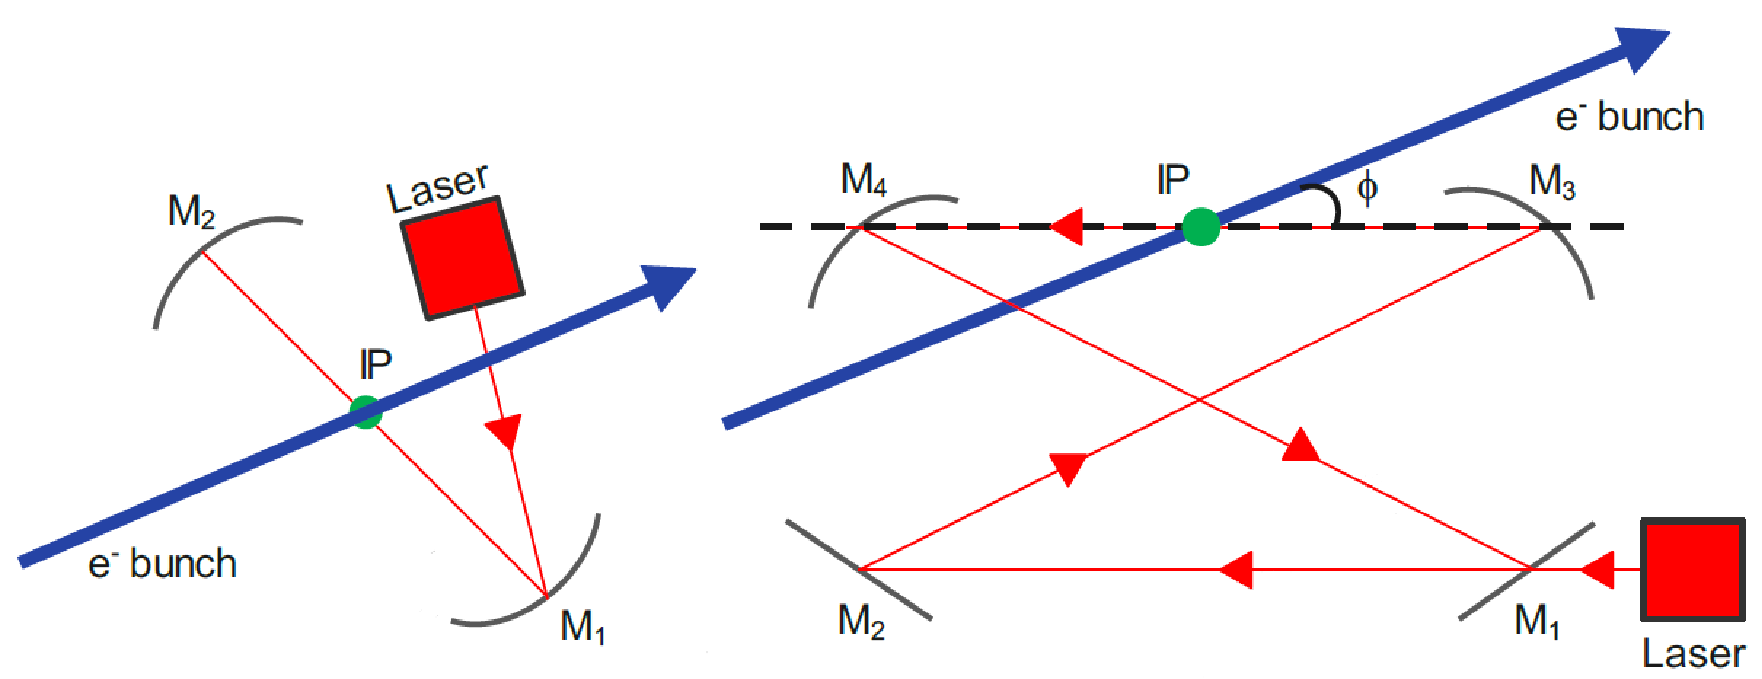
\includegraphics[width=\textwidth]{Figures/Photon_Production_by_Inverse_Compton_Scattering/2_mirror_4_mirror.pdf}
\caption{Fabry-Perot optical cavity constructed from varying amounts of mirrors where a laser (red) is circulated between the mirrors and interacted with an electron bunch (blue) at the interaction point (green). Left: 2 mirror Fabry-Perot optical cavity. Right: 4 mirror bow-tie Fabry-Perot optical cavity.}
\label{fig:2_mirror_4_mirror}
\end{figure}
As shown in Fig.~\ref{fig:2_mirror_4_mirror}, Fabry-Perot cavities typically exist in 4 mirror and 2 mirrror configurations. Two-mirror cavities consist of
two concave reflectors, requiring a concentric configuration to achieve a very small beam-waist, and are consequently mechanically very unstable \cite{dupraz2015abcd}. The concentric configuration is an extremely instable mode as displacements of the optical axis
correspond to small displacement on the mirrors \cite{variola2011luminosity} -- small cavity misalignments are poorly corrected by the optics. A comprehensive discussion of the mechanical instability of 2 mirror cavities and the difficulties associated with concentric configurations is presented by Zomer et al \cite{zomer2009polarization}, for there reasons only 4 mirror cavities are utilised here. 

The main advantages of using a Fabry--Perot optical cavity is that the average power of the incident laser can be increased as the repetition frequency can be increased from a standard CW laser and the cavity can accomodate a large number of passes of the stacked optical pulse \cite{variola2011luminosity}. Therefore, higher average laser powers -- the stored average laser power -- can be interacted with the high average power of a re-circulated electron bunch, with a higher interaction repetition rate, producing more inverse Compton scattering events. The average stored power of an optical cavity is given by
\begin{equation}
P_{\mathrm{avg}} = mE_{\mathrm{pulse}}f_{\mathrm{opt}},
\label{eq:average_stored_power_cavity}    
\end{equation}
where $m$ is the no. laser pulses stored in the cavity, $E_{\mathrm{pulse}}$ is the energy of the pulse stored in the cavity and $f_{\mathrm{opt}}$ is the repetition frequency of the laser in the optical cavity. Large laser infrastructure is also not required as the Fabry-Perot optical cavity typically re-circulates weak laser pulses, with pulse energies of 10--100's~\si{\micro\joule}. High average powers can be stored as the $\sim100$~\si{\micro\joule} pulse is re-circulated at 100's~\si{\mega\hertz} -- a typical electron bunch repetition frequency -- giving an average stored power of $P_{\mathrm{avg}}= 10$~\si{\kilo\watt}, much greater than the `single shot' approach where for Ti:Sa lasers the average power is 8.6~\si{\watt}.

However, implementation of Fabry-Perot cavities in an ICS source results in constraints to the path length, the angle of the interaction (crossing angle), the focal radius of the laser pulse at the interaction point and the average stored laser power available for interaction. These constraints on the optical cavity are interdependent, for example reducing the path length will reduce the energy of the pulse that can be stored for invariant laser average power.

The path length constraints arise due to the requirement that the electron bunch repetition rate and the laser pulse repetition rate must remain identical. Two conditions are imposed
\begin{align}
f_{\mathrm{electron}} &= mf_{\mathrm{opt}}, & L_{\mathrm{cav}} &= \frac{c}{f_{\mathrm{laser}}},
\label{eq:optical_path_length_conditions}    
\end{align}
where $f_{\mathrm{electron}}$ is the electron bunch repetition rate and $L_{\mathrm{cav}}$ is the path length of the cavity. A path length that is too large will amplify the effect of mirror misalignments as a ray incident on a misaligned mirror will have a larger positional error on the other cavity mirror is the distance between them is larger \cite{zomer2009polarization}. Small path lengths are unfeasible because the laser spot size upon the mirrors becomes too small, and the power of the laser pulse incident on cavity mirrors become above damage thresholds (see Section~\ref{sec:ICS_lasers}). The transverse \textit{rms} spot size of a laser pulse a distance $z_{L}$ from focus is given by \cite{siegmann1986lasers}
\begin{equation}
\sigma_{w} = \sigma_{L}\sqrt{1+\frac{z_{L}}{z_{R}}},
\label{eq:laser_waist}    
\end{equation}
with $\sigma_{L}$ the transverse \textit{rms} spot size of the laser pulse and the Rayleigh range \cite{siegmann1986lasers} of a laser pulse of wavelength $\lambda$ is
\begin{equation}
z_{R} = \frac{4\pi\sigma_{L}^{2}}{\lambda}.
\label{eq:rayleigh_range}    
\end{equation}

The spot size at the interaction point of a 4 mirror cavity, as shown in Fig.~\ref{fig:2_mirror_4_mirror}, can be made smaller by increasing the distance between the two curved cavity mirrors ($M_{3}$ and $M_{4}$), whilst maintaining their radius of curvature \cite{zomer2009polarization, akagi2016narrow}. The spot size on the $M_{3}$ and $M_{4}$ mirrors remains unchanged but, as seen through inspection of (Eq.~\ref{eq:laser_waist}), the spot size at the interaction point between these becomes smaller. Distances between the $M_{1}$ and $M_{2}$ mirrors are adjusted to maintain the path length requirements (Eq.~\ref{eq:optical_path_length_conditions}). Small laser pulse spot sizes at the IP are limited by misalignments of the optical cavity mirrors limiting the distance between the $M_{3}$ and $M_{4}$ mirrors and the closeness of the $M_{1}$ and $M_{2}$ mirrors is similarly limited by the damage thresholds of those mirrors.

A crossing angle of between 2--12\si{degree} is typically imposed between the electron bunch and the laser pulse in a Fabry-Perot optical cavity \cite{variola2011luminosity} to avoid the electron bunches impinging upon the optical mirrors, which would damage the mirror surfaces. Alternatively, two schemes could be used where a head-on ($\phi=0$) interaction is permissible. The electron bunch could be incident through a hole in the mirror, which reduces the reflection of the cavity mirrors and reduces the stored power, radiation damage could also occur from electron beam halo or miss steered electron beams. Or, the electron bunch could enter a large Fabry-Perot optical cavity via a chicane (see Section~\ref{sec:magnetic_bunch_compression}) avoiding the mirrors entirely, however magnets would then be placed within the optical cavity  which could compromise steering of
the laser beam by inducing thermal stress in the optics \cite{gunther2019device}.

The finesse of an optical cavity expresses the no. round trip passes a laser pulse can accomplish before being absorbed or lost by transmission through the cavity mirrors. Therefore, this is an important performance parameter of an optical cavity, analogous to the $Q$ of an RF cavity. The finesse of a Fabry-Perot optical cavity is given by \cite{ismail2016fabry}
\begin{equation}
F=\frac{\pi}{2\sin^{-1}\left(\frac{1-\sqrt{V}}{2\sqrt[4]{V}}\right)} \approx \frac{2\pi}{1-V},
\label{eq:finesse}    
\end{equation}
where $V$ is the fraction power loss per cavity round trip, and the approximation is valid for $V \ll 1$ i.e small round trip losses. For a input mirror with transmission $T_{1}$, the finesse becomes
\begin{equation}
F=\frac{2\pi T_{1}}{\left(T_{1}+V\right)^{2}}
\label{eq:fabry_perot_finesse}    
\end{equation}
Consequently, a high finesse cavity is necessary to being able to transport a high average stored power otherwise power losses on the mirrors and mirror heating would become prohibitive. A high average power on the cavity mirrors heats the mirrors locally, which causes thermoelastic deformation of the mirrors and affects their radii of curvature preventing good coupling of the laser pulse to the cavity \cite{chaikovska2016high}, thereby causing greater power loss, which reinforces this behaviour -- the cavity eventually becomes unstable. However, mitigation of thermoelastic deformation of optical mirrors in Fabry-Perot optical cavities is an active research subject \cite{amoudry2020modal}.  A high average power also means a cavity is more susceptible to hot-spot defects, where defects on a mirror surface cause a hot-spot and the mirror coating is damaged resulting in a large loss of stored power \cite{wang2020prior}. Limitations on the average stored power within an optical cavity mean that the multi-pulse optical cavity approach (where $m$ pulses are re-circulated) is not advantageous to increasing the scattered photons produced by the ICS source because the energy of the pulses in the optical cavity must be decreased due to the number of pulses in the cavity i.e $E_{pulse}/m$.    

\section{Non-linear Inverse Compton Scattering}
\label{sec:nonlinear_ICS}

The inverse Compton scattering process becomes non-linear when the the scattering is performed with a particularly intense source of incident photons. In inverse Compton scattering sources, where the scope of this work lies, the source of photons is commonly a laser pulse, as explained in Section~\ref{sec:lasers_fabry_perot}. The intensity of the incident photon source is typically characterised using the normalised laser vector potential $a_{0}$ which can be defined for both a Gaussian (Eq.~\ref{eq:a0_gaussian}) and flat-top (Eq.~\ref{eq:a0_flat_top}) pulse \cite{terzic2019improving}
\begin{align}
a_{0} &= \frac{e\sqrt{2c\mu_{0}}}{2\pi m_{e}c^{2}}\lambda\sqrt{\frac{E_{\mathrm{pulse}}}{\left(2\pi\right)^{3/2}\sigma_{L}^{2}t_{\mathrm{pulse}}}},
\label{eq:a0_gaussian} \\
a_{0} &= \frac{e\sqrt{2c\mu_{0}}}{2\pi m_{e}c^{2}}\lambda\sqrt{\frac{E_{\mathrm{pulse}}}{2\pi\sigma_{L}^{2}t_{\mathrm{pulse}}}},
\label{eq:a0_flat_top}
\end{align}
where $e$ is the charge of an electron, $\mu_{0}$ is the permeability of free space, $E_{\mathrm{pulse}}$ is the energy of the incident photon pulse, $\sigma_{L}$ is the transverse \textit{rms} spot size (radius) of the incident photon pulse and $t_{pulse}$ is the \textit{rms} pulse duration. The normalised laser potential is sometimes expressed more empirically by $a_{0} \approx 0.855\times 10^{-9} \lambda\left[\mathrm{\mu m}\right]\sqrt{I\left[\mathrm{W/cm^{2}}\right]}$, where $I$ is the intensity of the incident photon pulse \cite{li2004high}.

When $a_{0} \ll 1$ the inverse Compton scattering interaction is termed linear, once this limit is encroached non-linear effects begin to have an effect on an inverse Compton scattering source. Common effects are ponderomotive broadening of the resulting spectra \cite{krafft2004spectral}, harmonic generation of higher energy photons cite{sarachik1970classical,babzien2006observation} and multi-photon inverse Compton scattering \cite{bula1996observation}. Ponderomotive broadening and harmonic generation effects are possible with $a_{0}<1$ as their onset is also driven by other factors such as pulse length and shape, but for multi-photon inverse Compton scattering $a_{0}>1$. Unless explicitly stated, all equations within this work are derived for the linear regime as this is the regime the ICS sources presented are designed to operate.

% Ponderomotive Broadening
Ponderomotive broadening is a form of spectral broadening caused by the ponderomotive force of the incident photon pulse acting upon the electron bunch. During a laser pulse - electron beam interaction, the electron is decelerated, then accelerated by the ponderomotive force of the laser
pulse. These velocity shifts lead to frequency shifts in the
emitted radiation, increasing the width of the observed
spectrum \cite{krafft2004spectral}. The broadening effect is visible in the radiation emitted from each laser harmonic. Ponderomotive broadening is therefore a detrimental effect to the pursuit of quasi-monochromatic high-intensity photon beams, which are most favoured by radiation users. 

% Ponderomotive Broadening Mitigation
Hence, mitigation of ponderomotive effects is an extensively studied topic \cite{ghebregziabher2013spectral,terzic2014narrow,seipt2015narrowband,rykovanov2016controlling,terzic2016combining,terzic2019improving}. Strategies to mitigate ponderomotive broadening frequently involve the 'chirping' or frequency modulation of the laser pulse, in which the laser pulse shape is controlled in order to minimize the deceleration and acceleration of the interacted electrons. This is analagous to undulator tapering in free electron lasers The local $a_{0}$ of the laser pulse is modulated by the shape of the pulse in order to accomplish control of the ponderomotive force. 

The laser chirp can be produced with conventional stretcher/compressor and pulse-shaper combinations \cite{ghebregziabher2013spectral}, i.e using existing conventional laser optics or via an FEL oscillator, where the substatial bunch length of the driving electron bunches are of a length where the RF-curvature energy spread is considerable, which means that the resulting laser pulse emitted by the FEL will
also be chirped \cite{terzic2014narrow}. Solutions have been derived for a range of pulse shapes and modulation schemes up to a full 3D laser pulse description \cite{terzic2019improving}, however the chirping ponderomotive broadening mitigation technique is yet to be experimentally demonstrated.

% Harmonic Generation
Harmonic generation is the non-linear inverse Compton scattering process in which the incident electron is accelerated by the electromagnetic field of the incident laser pulse. Anharmonic acceleration of the electron, as it interacts with the radiation field \cite{englert1983second}, causes non-sinusoidal transverse oscillations of the electron and induced figure-8 motion, which introduces an overall redshift in the radiation
spectrum, with the concomitant emission of higher order harmonics \cite{sakai2015observation}. The electrodynamics of harmonic generation by free electrons was first described quantum mechanically by Brown and Kibble \cite{brown1964interaction,kibble1965frequency} with a following classical interpretation by Sarrachik and Schappert \cite{sarachik1970classical}. 

The harmonic generation effect at the second harmonic was said to be demonstrated in 1983 \cite{englert1983second}, however the authors could not confirm whether this was harmonic generation or multi-photon inverse Compton scattering. Subsequently, confirmation of harmonic generation was first achieved at Brookhaven National Laboratory \cite{babzien2006observation,kumita2006observation} using a 60~\si{\mega\electronvolt} electron bunch in a head-on interaction with a CO$_{2}$ laser ($\lambda = 10.6$~\si{\micro\meter}) at a normalised laser vector potential of $a_{0} = 0.35$. The scattered photon beam generated at the BNL ATF contained both the fundamental harmonic, at an energy of $E_{\gamma} = 6.5$~\si{\kilo\electronvolt}, and the second harmonic with a peak energy of $E_{\gamma} = 13$~\si{\kilo\electronvolt}, if $a_{0}$ was larger we would expect to see increasingly large red-shifting of the scattered photon energy of each harmonic \cite{kibble1965frequency,sakai2015observation} as well as the standard recoil reduction beyond the Thomson regime ($1 \ll 1$). The doubling of the scattered photon energy arises due to the electron oscillating and double the laser frequency of the fundamental harmonic. To observe the 2nd harmonic, the fundamental harmonic must be filtered via attenuation in a silver foil \cite{babzien2006observation}, which attenuates the fundamental spectrum to a larger extent because of the lower photon energy.

However, the Ag foil filtering will not completely remove the fundamental harmonic, instead the transverse profile of the filtered scattered photon beam is imaged via a luminescent screen. For the second harmonic radiation a set of two off-axis intensity peaks will be observed, unlike the fundamental harmonic which shows a central intensity peak. The double peak phenomena occurs because the $\overrightarrow{v}\times\overrightarrow{B}$ term of the Loretz force of the laser pulse is comparable to the electric field term which causes an electron to oscillate in the laser field at a higher frequency, with a characteristic figure of 8 transverse motion \cite{sarachik1970classical,jackson1999classical} in the electron frame, thereby modifying the angular intensity distribution of the produced radiation from a $\sin^{2}\theta$ dependence for the fundamental harmonic to a $\cos^{2}\theta$ dependence for the second harmonic which upon transformation to the lab frame results in the double peak behaviour \cite{babzien2006observation}. The double intensity peaks for the second harmonic are separated by an angle $\Delta\theta = 1/\gamma$.   

% Multi-Photon Compton Scattering
Alternatively, the non-linear inverse Compton scattering process can be thought of as the simultaneous interaction of multiple incident photons with an electron and the corresponding scattering of these as a single photon. The general equation for a multi-photon interaction, modified from (Eq.~\ref{eq:ICS_process}) \cite{bula1996observation,seipt2011nonlinear}
\begin{equation}
p_{1} + \mathit{n}k_{1} = p_{2} + k_{2},
\label{eq:nonlinear_electron_photon_interaction}    
\end{equation}
where $n$ denotes an integer value of incident photons present in the interaction. As we have two or more identical photons interacting simultaneously, the total incident photon energy is $n E_{L}$ and consequently the scattered photon energy is roughly $nE_{\gamma}$, this is not the case because of redshifting and increased recoil, as discussed previously. Demonstration of a multi-photon inverse Compton scattering source by C. Bula et al \cite{bula1996observation} at the Final Focus Test Beam at SLAC \cite{burke1994results} showed an inverse Compton scattering  interaction with 4 incident photons, using a high intensity laser pulse. Therefore, high harmonics can be achieved via this interaction. 

The terms harmonic generation and multi-photon ICS are used interchangeably within the literature \cite{}, however these both encompass an identical process. Harmonic generation is typically favoured terminology by those utilising classical methods to explain the behaviour whilst multi-photon inverse Compton scattering is used when the full quantum mechanical interpretation is used. The classical theory \cite{sarachik1970classical} allows for the coarse features of the behaviour such as the figure 8 motion of the electrons in the high field pulse and the angular distribution of emission to be understood whilst the quantum treatment \cite{brown1964interaction,kibble1965frequency} allows the description of morel subtle features such as the spin effects of the interaction.    

\section{Derivation of the Scattered Photon Energy}
\label{sec:derivation_of_the_scattered_photon_energy}

The relation in (Eq.~\ref{eq:ICS_process}) can be modified in order to calculate the scattered photon energy of an electron - photon interaction. Using the four-momenta in (Eq.~\ref{eq:initial_four_vectors}-\ref{eq:final_four_vectors}) we can create Lorentz invariant quantities from the Minkowski norms of the four-momenta 
\begin{align}
p_{1\mu}p_{1}^{\mu} &= \gamma^{2}m_{e}^{2}\left(v^{2}-c^{2}\right) = -m_{e}^{2}c^{2},
\label{eq:lorentz_invariants1} \\
k_{1\mu}k_{1}^{\mu} &= 0.
\label{eq:lorentz_invariants2}
\end{align}

We can multiply (Eq.~\ref{eq:ICS_process}) by the four-momentum  of the scattered photon and apply (Eq.~\ref{eq:lorentz_invariants2}) the Lorentz invariant 
\begin{align}
k_{2}^{\mu}\left(p_{1\mu} + k_{1\mu}\right) &= k_{2}^{\mu}\left(p_{2\mu} + k_{2\mu}\right), \\
k_{2}^{\mu}p_{1\mu}+k_{2}^{\mu}k_{1\mu} &= k_{2}^{\mu}p_{2\mu}.
\label{eq:apply_photon_pfinal}
\end{align}

Similarly we can construct another equation by inspecting the square of the conservation of four-momentum
\begin{align}
\left(p_{1}+k_{1}\right)_{\mu}\left(p_{1}+k_{1}\right)^{\mu} &= \left(p_{2}+k_{2}\right)_{\mu}\left(p_{2}+k_{2}\right)^{\mu}, \\
p_{1\mu}p_{1}^{\mu}+k_{1\mu}p_{1}^{\mu}+k_{1\mu}p_{1}^{\mu}+k_{1\mu}k_{1}^{\mu} &= p_{2\mu}p_{2}^{\mu}+k_{2\mu}p_{2}^{\mu}+p_{2\mu}k_{2}^{\mu}+k_{2\mu}k_{2}^{\mu},
\label{eq:apply_conservation_squared}
\end{align}
utilising the commutation of four-vectors ($p_{\mu}k^{\mu} = k_{\mu}p^{\mu}$) and our Lorentz invariants (Eq.~\ref{eq:lorentz_invariants1}, \ref{eq:lorentz_invariants2}) we can simplify this further 
\begin{equation}
p_{1\mu}k_{1}^{\mu} = p_{2\mu}k_{2}^{\mu}.
\label{eq:end_conservation_squared}
\end{equation}
Subbing (Eq.~\ref{eq:end_conservation_squared}) into (Eq.~\ref{eq:apply_photon_pfinal}) yields
\begin{equation}
k_{2}^{\mu}p_{1\mu}+k_{2}^{\mu}k_{1\mu} = k_{1}^{\mu}p_{1\mu}
\label{eq:substitution_four_vector}
\end{equation}

Which in three-vector notation is shown as
\begin{equation}
\frac{E_{L}E_{\gamma}}{c^{2}}\left(\hat{n}_{i}\cdot\hat{n}_{f}-1\right)+\frac{E_{\gamma}}{c}\gamma m_{e}\left(\hat{n}_{f}\cdot \boldsymbol{v_{i}}-c\right) = \frac{E_{L}}{c}\gamma m_{e}\left(\hat{n}_{i}\cdot \boldsymbol{v_{i}} -c\right)
\label{eq:three_vector_solution}
\end{equation}

However, (Eq.~\ref{eq:three_vector_solution}) should be presented in terms of the angles in Fig.~\ref{fig:scattered_photon_kinematics}. The dot products within this formula can be replaced using projections to introduce the angular dependencies
\begin{align}
\hat{n}_{i}\cdot\hat{n}_{f} &= \cos\theta',
\label{eq:projection_angle_incident_scattered_photon}\\
\hat{n}_{f}\cdot \boldsymbol{v_{i}} &= v_{i}\cos\theta,
\label{eq:projection_scattering_angle}\\
\hat{n}_{i}\cdot \boldsymbol{v_{i}} &= v_{i}\cos\phi'.
\label{eq:projection_pi_minus_crossing_angle}
\end{align}

Upon introducing the projections (Eq.~\ref{eq:projection_angle_incident_scattered_photon}, \ref{eq:projection_scattering_angle}, \ref{eq:projection_pi_minus_crossing_angle}), (Eq.~\ref{eq:three_vector_solution}) becomes
\begin{equation}
E_{L}E_{\gamma}\left(\cos\theta'-1\right)+E_{\gamma}\gamma m_{e}c^{2}\left(\frac{v_{i}}{c}\cos\theta-1\right) = E_{L}\gamma m_{e}c^{2}\left( \frac{v_{i}}{c}\cos\phi'-1\right)
\label{eq:three_vector_solution_projections}
\end{equation}
Using the Lorentz speed factor $\beta = v/c$ and the total electron beam energy $E_{e} = \gamma m_{e}c^{2}$ and rearranging we arive at the general linear, recoil-corrected form for the scattered photon energy resulting from inverse Compton scattering 
\begin{equation}
E_{\gamma} = \frac{\left(1-\beta\cos\phi'\right)E_{L}}{1-\beta\cos\theta+\left(1-\cos\theta'\right)\frac{E_{L}}{E_{e}}}. 
\label{eq:scattered_photon_energy}
\end{equation}
  
In the head-on case ($\phi=0$), (Eq.~\ref{eq:scattered_photon_energy}) can be simplified to 
\begin{equation}
E_{\gamma} = \frac{\left(1+\beta\right)}{1-\beta\cos\theta-\left(\beta-E_{L}/E_{e}\right)\cos\theta},
\label{eq:headon_scattered_photon_energy}
\end{equation}
further simplification by the small angle approximation ($\theta \ll 1$) and for an ultra-relativistic electron beam ($\beta \rightarrow 1$) yields
\begin{equation}
E_{\gamma} \approx \frac{4\gamma^{2}E_{L}}{1+\gamma^{2}\theta^{2}+X},    
\label{eq:small_angle_scattered_photon_energy}
\end{equation}
where the recoil term $X$ is given by (Eq.~\ref{eq:X_headon}). Extending this to backscattering of the incident photon ($\theta = 0$), the scattered photon energy becomes
\begin{equation}
E_{\gamma} = \frac{4\gamma^{2}E_{L}}{1+X},
\label{eq:headon_backscattering_scattered_photon_energy}
\end{equation}
which is referred to in the literature \cite{krafft2010compton} as the Compton edge. The $\gamma^{2}$ factor within this equation refers to the double Doppler shift experienced by the incident photon as it is scattered. At low recoil the Compton edge energy is given by the well known relation
\begin{equation}
E_{\gamma} = 4\gamma^{2}E_{L}.
\label{eq:compton_edge_energy}    
\end{equation}

Upon inspection of the generalised ICS scattered photon energy (Eq.~\ref{eq:scattered_photon_energy}), there is an explicit dependence of the scattering angle and therefore the scattered photon energy is proportional to the scattered photon energy ($E_{\gamma} \propto \theta$). The energy--angle correspondence of the scattering interaction enables scattered photon energy selection via specification of a maxmimum opening angle the radiation can traverse -- the produced radiation can be simply collimated.   

\section{Electron - Photon Interaction Cross Section}
\label{sec:electron_photon_interaction_cross_section}

To understand the cross section of the interaction the interaction must be viewed three dimensionally and considerations such as polarisation must be adequately accounted for. The co-ordinate system in Fig.~\ref{fig:scattered_photon_kinematics} can be extended to a full 3D representation in Fig.~\ref{fig:3D_coord_system}, with an incident electron $p_{1}$ parallel to the $z$-axis interacting with an incident photon $k_{1}$ travelling anti-parallel, with a crossing angle $\phi$ in the $x$-$z$ plane, scattering a photon $k_{2}$ at a polar angle $\theta$ and azimuthal angle $\phi_{f}$. Whilst the incident electron is used to set the right-handed global co-ordinate system ($x$, $y$, $z$), local right-handed co-ordinate systems can be attached to the incident photon ($\tilde{x}$, $\tilde{y}$, $\tilde{z}$), which propagates anti-parallel to the electron at a crossing angle $\phi$ ($x = -\tilde{x}\sin\phi$, $z = -\tilde{z}$), and to the scattered photon ($\tilde{x}'$,$\tilde{y}'$,$\tilde{z}'$) where the variation from the electron co-ordinate system is due to the polar scattering angle $\theta$. Polarisation directions of the incident and scattered photons is typically specified in the local co-ordinate systems.  

\begin{figure}[!h]
\centering
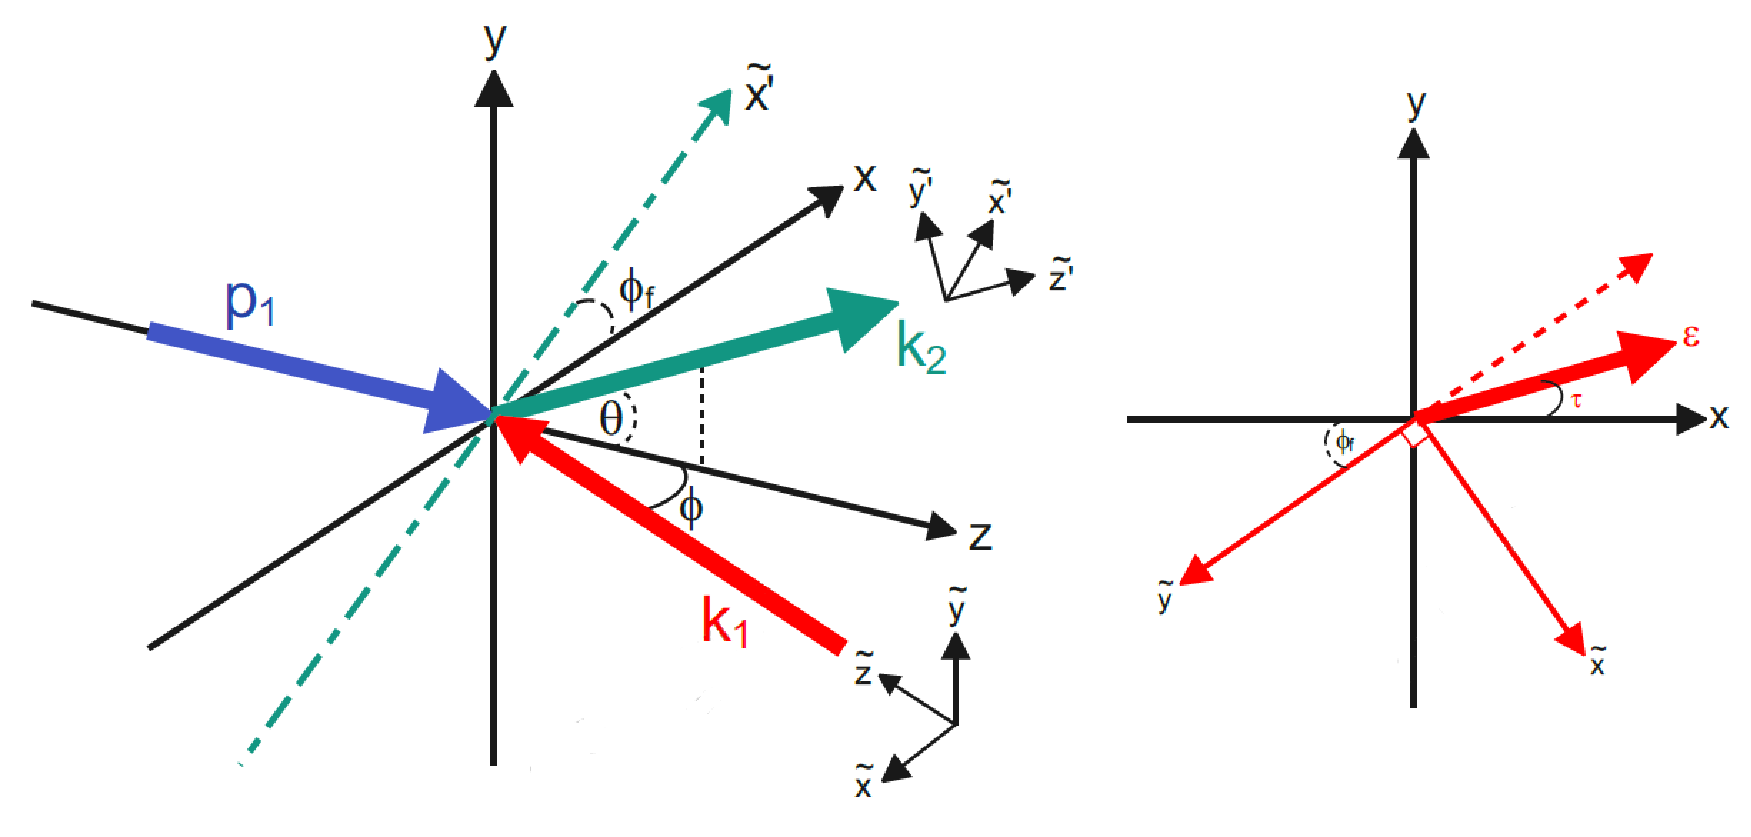
\includegraphics[width=\textwidth]{Figures/Photon_Production_by_Inverse_Compton_Scattering/ICS_interaction_polarisation.pdf}
\caption{Diagram of the electron--photon scattering interactions. Left: Geometry of the interaction in the incident electron global co-ordinate system. An incident electron (blue) with momentum $p_{1}$ interacts with an incident photon (red) with momentum $\hbar k_{1}$ at a crossing angle $\phi$ in the $x$--$z$ plane and rotated in the $x$--$y$ plane by azimuthal angle $\phi_{f}$. The photon is scattered (green) with momentum $\hbar k_{2}$ at a polar scattering angle $\theta$ in the $y$--$z$ plane with azimuthal angle $\phi_{f}$. The incident and scattered photons have local right handed co-ordinate systems attached.  Right: Polarisation vector $\varepsilon$ (red) of the incident linearly polarised photon with reference to the local co-ordinate system (red) and electron frame (black). The incident photon travels into the page, with the aximuthal angle of linear polarisation $\tau$ defined with reference to the $x$ axis of the electron frame.}
\label{fig:3D_coord_system}
\end{figure}

Following the derivation by Berestetskii, Lifshitz and Pitaevskii \cite{berestetskii1982quantum}, using the amplitude arising from the Feynman diagrams in Fig.~\ref{fig:ICS_Feynman_diagrams}, the double differential cross section with respect to any polarisation of the incident and scattered photons and an unpolarised or arbitrarily polarised electron is given by 
\begin{multline}
\frac{d^{2}\sigma}{dYd\phi_{f}} = \frac{2r_{e}^{2}}{X}\left\{\left(\frac{1}{X}-\frac{1}{Y}\right)^{2}+\frac{1}{X}-\frac{1}{Y}+\frac{1}{4}\left(\frac{X}{Y}+\frac{Y}{X}\right)  -\left(\xi_{3}+\xi_{3}'\right)\left[\left(\frac{1}{X}-\frac{1}{Y}\right)^{2}+\frac{1}{X}-\frac{1}{Y}\right] \right.\\\left. +\xi_{1}\xi_{1}'\left(\frac{1}{X}-\frac{1}{Y}+\frac{1}{2}\right) + \xi_{2}\xi_{2}'\left[\frac{1}{4}\left(\frac{X}{Y}+\frac{Y}{X}\right)\left(1+\frac{2}{X}-\frac{2}{Y}\right)\right] \right.\\\left. + \xi_{3}\xi_{3}'\left[\left(\frac{1}{X}-\frac{1}{Y}\right)^{2}+\frac{1}{X}-\frac{1}{Y}+\frac{1}{2}\right] \right\}
\label{eq:polarisation_differential_cross_section}    
\end{multline}
where the incident photon pulse Stokes parameters $\xi_{i}$, in the electron frame (global) co-ordinate system, are given by
\begin{align}
\xi_{1} &= P_{t}\sin\left(2\tau-2\phi_{f}\right)\sin\phi\\
\xi_{2} &= P_{c} \\
\xi_{3} &= -P_{t}\cos\left(2\tau-2\phi_{f}\right)\sin\phi
\label{eq:incident_stokes_parameters}    
\end{align}
where, using the same co-ordinate system as Sun and Wu \cite{sun2009characterizations,sun2011theoretical}, $-1 \geq P_{t} \geq 1$ is the degree of linear polarisation of the incident pulse ($P_{t}=-1$, full anti-parallel polarisation), $-1 \geq P_{c} \geq 1$ is the degree of circular polarisation of the incident pulse ($P_{c}=-1$, full anticlockwise polarisation), $\tau$ is the azimuthal angle of the linear polarisation, $\phi_{f}$ is the azimuthal scattering angle, $\phi$ is the crossing angle in the $x$--$z$ plane.

The Stokes parameters $\xi'$ of a single scattered photon  for a small polar scattering angle ($\theta \ll 1$) in the electron frame can be similarly defined
\begin{align}
\xi'_{1} &\approx -\bar{\xi'_{1}}\cos\left(2\phi_{f}\right)+\bar{\xi'_{3}}\sin\left(2\phi_{f}\right), \\
\xi'_{2} &\approx \bar{\xi'_{2}}, \\
\xi'_{3} &\approx -\bar{\xi'_{1}}\sin\left(2\phi_{f}\right)-\bar{\xi'_{3}}\cos\left(2\phi_{f}\right),
\end{align}
where $\bar{\xi'_{i}}$ are the scattered photon Stokes parameters of the scattered photon in its attached local co-ordinate system. For example $\bar{xi'_{i}} = \left(0, 0, 1\right)$, corresponds to a horizontally polarised scattered photon aligned to $\tilde{x}$. 

Assuming, for the purposes of a general cross section formula, ambivalence over the polarisation state of the scattered photons i.e scattered photons are not discriminated on the basis of polarisation from an ICS interaction, the cross section can be derived by setting $\xi_{i}' = 0 ~\left(i=1,~2,~3\right)$. Making this assumption, the double differential cross section (Eq.~\ref{eq:polarisation_differential_cross_section}) reduces to
\begin{equation}
\frac{d^{2}\sigma}{dYd\phi_{f}} =  \frac{4r_{e}^{2}}{X^{2}}\left[1+P_{t}\cos\left(2\tau-2\phi_{f}\right)\right]\left\{\left(1-\xi_{3}\right)\left[\left(\frac{1}{X}-\frac{1}{Y}\right)^{2}+\frac{1}{X}-\frac{1}{Y}\right]+\frac{1}{4}\left(\frac{X}{Y}+\frac{Y}{X}\right)\right\},
\label{eq:double_differential_cross_section}    
\end{equation}
Integrating over the full range of the azimuthal scattering angle $0 \leq \phi_{f} \leq 2\pi$ obtains the differential cross section as a function of the $Y$ Lorentz invariant (Eq.~\ref{eq:Y_geometry}) 
\begin{align}
 \frac{d\sigma}{dY} &= A\int_{0}^{2\pi}1+P_{t}\cos\left(2\tau-2\phi_{f}\right\sin\phi~d\phi_{f}+ B\int_{0}^{2\pi}~d\phi_{f}, \nonumber \\
 \frac{d\sigma}{dY} &= 2\pi\left(A+B\right) = \frac{8\pi r_{e}^{2}}{X^{2}}\left[\left(\frac{1}{X}-\frac{1}{Y}\right)^{2}+\frac{1}{X}-\frac{1}{Y}+\frac{1}{4}\left(\frac{X}{Y}+\frac{Y}{X}\right)\right],
\label{eq:differential_cross_section_Y_invariant}
\end{align}
where $A$ and $B$ parameterise $\phi_{f}$ independent parameters in (Eq.~\ref{eq:double_differential_cross_section}) given by
\begin{align}
A &= \frac{4r_{e}}{X^{2}}\left[\left(\frac{1}{X}-\frac{1}{Y}\right)^{2}+\frac{1}{X}-\frac{1}{Y}\right], \nonumber\\
B &= \frac{4r_{e}^{2}}{X^{2}}\left[\frac{1}{4}\left(\frac{X}{Y}+\frac{Y}{X}\right)\right].
\label{eq:phif_independent_parameters}
\end{align}
Through inspection of (Eq.~\ref{eq:differential_cross_section_Y_invariant}), it is clear there is no longer a dependence on the polarisation of the incident photon therefore, the flux of an ICS interaction is independent of the polarisation of the incident photons.

Following the derivation of Berestetskii \cite{berestetskii1982quantum}, the Mandelstam variables for the electron--photon interaction are limited by $s\geq m_{e}c^{2}$, $t \leq 0$ and $u s \leq \left(m_{e}c^{2}\right)^{2}$ which can be rearranged to form the inequality $\frac{X}{X+1} \leq Y \leq X$ \cite{sun2009characterizations}. The total cross section for the inverse Compton scattering interaction \cite{berestetskii1982quantum} can be integrated within the range of the inequality
\begin{align}
\sigma &= \frac{8\pi r_{e}^{2}}{X^{2}}\int_{\frac{X}{X+1}}^{X}\left(\frac{1}{X}-\frac{1}{Y}\right)^{2}+\frac{1}{X}-\frac{1}{Y}+\frac{1}{4}\left(\frac{X}{Y}+\frac{Y}{X}\right)~dY, \nonumber \\
\sigma &= \frac{2\pi r_{e}^{2}}{X}\left[\frac{1}{2}+\frac{8}{X}-\frac{1}{2\left(1+X\right)^{2}}+\left(1-\frac{4}{X}-\frac{8}{X^{2}}\right)\ln{\left(1+X\right)}\right],
\label{eq:compton_cross_section}
\end{align}
where $r_{e}$ is the classical radius of the electron. If, as in Curatolo et al \cite{curatolo2017analytical}, we take the classical limit ($X \to 0$) of the total cross section (Eq.~\ref{eq:compton_cross_section}) we obtain
\begin{equation}
\lim_{X \to ~0} \sigma = \frac{8\pi r_{e}^{2}}{3}\left(1-X\right) = \sigma_{T}\left(1-X\right),
\label{eq:compton_cross_section_classical_limit}
\end{equation}
where $\sigma_{T}$ is the Thomson cross section. Where the interaction is firmly in the classical regime ($X \ll 1$), in which inverse Compton scattering becomes Thomson scattering and there is elastic scattering, the Compton cross section recovers the Thomson scattering cross section, $\sigma = \sigma_{T}$. If we take the ultra-relativistic limit ($X \to \infty$) of (Eq.~\ref{eq:compton_cross_section}), the cross section becomes
\begin{equation}
\lim_{X \to ~\infty} \sigma = \frac{2\pi r_{e}^{2}}{X}\left(\ln{X}+\frac{1}{2}\right).
\label{eq:compton_cross_section_ultrarelativistic_limit}
\end{equation}

\begin{figure}[!h]
\centering
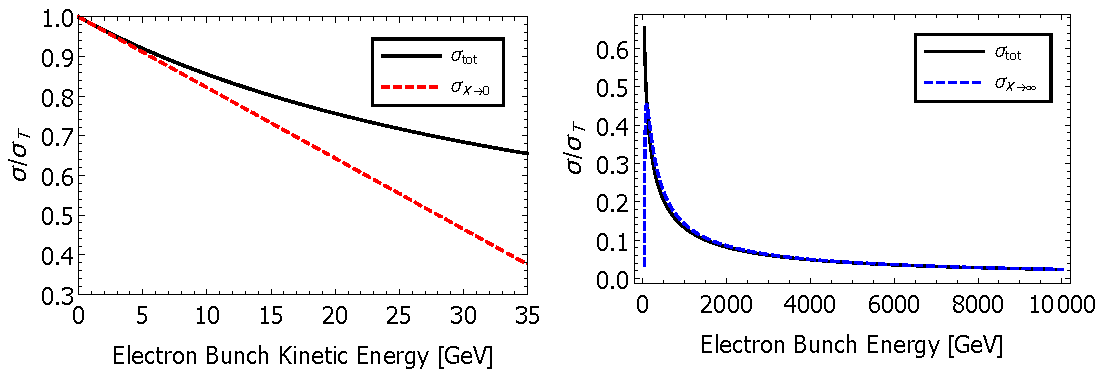
\includegraphics[width=\textwidth]{Figures/Photon_Production_by_Inverse_Compton_Scattering/Cross_Section_Electron_Bunch_Energy_NDYAG.pdf}
\caption{Electron--Photon interaction cross section (Eq.~\ref{eq:compton_cross_section}) as a function of electron bunch energy for an Nd:YAG laser operating at the fundamental harmonic ($\lambda = 1064$~\si{\nano\meter}). Left: Comparison of the full cross section (Eq.~\ref{eq:compton_cross_section}) (black) with the cross section in the low recoil limit (Eq.~\ref{eq:compton_cross_section_classical_limit}) (red) for a 5~\si{\mega\electronvolt}--35~\si{\giga\electronvolt} electron bunch kinetic energy range. Right: Comparison of the full cross section (Eq.~\ref{eq:compton_cross_section}) with the cross section in the ultra-relativistic, high recoil limit (Eq.~\ref{eq:compton_cross_section_ultrarelativistic_limit}) (blue) for a 35~\si{\giga\electronvolt}--10~\si{\terra\electronvolt} electron bunch kinetic energy range.}
\label{fig:cross_section_electron_energy}
\end{figure}

The behaviour of the total cross section as a function of electron bunch energy is shown in Fig.~\ref{fig:cross_section_electron_energy}. Fig.~\ref{fig:cross_section_electron_energy} shows that a small recoil ($X \ll 1$) cross section calculation is valid up until the \si{\giga\electron}-scale, above the \si{\giga\electronvolt}-scale the small recoil approximation (Eq.~\ref{eq:compton_cross_section_classical_limit}) underestimates the electron--photon interaction cross section (Eq.~\ref{eq:compton_cross_section}). The ultra-relativistic cross section approximation (Eq.~\ref{eq:compton_cross_section_ultrarelativistic_limit}) becomes a good approximation to the full cross section calculation (Eq.~\ref{eq:compton_cross_section}) beyond  $\sim92$~\si{\giga\electronvolt}, at smaller energies the cross section is underestimated and at energies on the order of 100's~\si{\giga\electronvolt} the cross section in the ultra-relativistic approximation is negative which is clearly nonphysical.     

Assuming a head-on ($\phi=0$) interaction in the ultra-relativistic domain ($\beta\approx1$) the Lorentz invariants can be related via
\begin{equation}
Y = X\frac{E_{e}-E_{\gamma}}{E_{e}-E_{L}},
\label{eq:lorentz_relation_headon_backscatter}
\end{equation}
where the derivative of $Y$ with respect to scattered photon energy becomes
\begin{equation}
\frac{dY}{dE_{\gamma}} = -\frac{X}{E_{e}-E_{L}}.
\label{eq:differential_lorentz_relation_headon_backscatter}
\end{equation}
The derivative of $Y$ with respect to the scattered photon energy $E_{\gamma}$ (Eq.~\ref{eq:differential_lorentz_relation_headon_backscatter}) is substituted into $d\sigma/dYd\phi_{f}$ (Eq.~\ref{eq:double_differential_cross_section}), which is integrated over the azimuthal angle, similarly to (Eq.~\ref{eq:differential_cross_section_Y_invariant}) to obtain the differential cross section with respect to the scattered photon energy
\begin{equation}
\frac{d\sigma}{dE_{\gamma}} = \frac{8\pi r_{e}^{2}}{X\left(E_{e}-E_{L}\right)}\left[\left(\frac{1}{X}-\frac{1}{Y}\right)^{2}+\frac{1}{X}-\frac{1}{Y}+\frac{1}{4}\left(\frac{X}{Y}+\frac{Y}{X}\right)\right].
\label{eq:differential_cross_section_ICS_energy}    
\end{equation}

Since the differential cross section can be wrote in terms of the scattered photon energy (Eq.~\ref{eq:scattered_photon_energy}), there is a cross section--scattering angle correspondence indirectly resulting from the scattered photon energy. The cross section--scattering angle correspondence from the scattered photon energy is also convoluted with the scattering angle dependency of the $Y$ Lorentz invariant (Eq.~\ref{eq:Y_geometry}). A full treatment of collimation and the differential cross section with respect to scattering angle is included in Chapter~\ref{Optimisation_and_Characterisation_of_Inverse_Compton Scattering_Spectra}, where the angular solutions are used to derive an analytical model for the collimated flux of an ICS interaction.    
The scattered photon energy differential cross section (Eq.~\ref{eq:differential_cross_section_ICS_energy}) can be plotted against the scattered photon energy of a single particle ICS interaction to reveal the spectral characteristics of an ICS source. Fig.~\ref{fig:cross_section_scattered_photon_energy} shows a normalised plot of the scattered photon energy differential cross section (Eq.~\ref{eq:differential_cross_section_ICS_energy}) as a function of the scattered photon energy for a head-on collision ($\phi=0$), in the low recoil regime ($X \ll 1$). Several features are apparent in Fig.~\ref{fig:cross_section_scattered_photon_energy}, such as the double peaked spectrum -- which is peaked in the forward (low energy) and backward (high energy) directions with respect to the scattered photon bunch -- where the intensity of these peaks is double (for $X \ll 1$) the intensity of the trough at $\theta=1/\gamma$ and the average energy ($E_{\gamma} = 2\gamma^{2}E_{L}$), which is half of the maximum energy (Eq.~\ref{eq:compton_edge_energy}) at the Compton edge.   

\begin{figure}[!h]
\centering
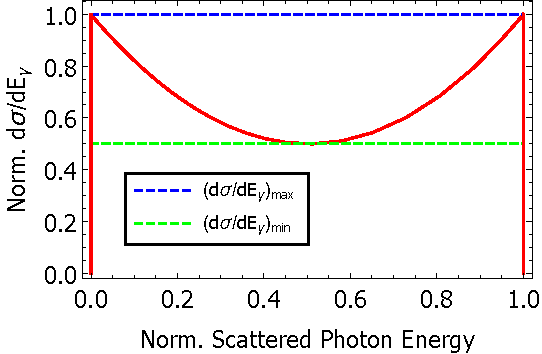
\includegraphics[width=0.6\textwidth]{Figures/Photon_Production_by_Inverse_Compton_Scattering/Cross_Section_Scattered_Photon_Energy.pdf}
\caption{Differential cross section with respect to the scattered photon energy (Eq.~\ref{eq:differential_cross_section_ICS_energy}) as a function of scattered photon energy (Eq.~\ref{eq:scattered_photon_energy}) in the low recoil ($X \ll 1$) regime for a head-on interaction ($\phi=0$), both parameters are normalised for generality. The maximum (blue) and minimum (green) values of the differential cross section (Eq.~\ref{eq:max_min_differential_cross_section_ICS_energy}) are shown, which differ by a factor of $\sim2$ (Eq.~\ref{eq:max_min_cross_section_ratio}).The average energy in the spectrum is $E_{\gamma}=2\gamma^{2}E_{L}$, half of the Compton edge energy (Eq.~\ref{eq:compton_edge_energy}), due to the symmetry of the spectrum.}
\label{fig:cross_section_scattered_photon_energy}
\end{figure}

Limitations of the Lorentz $Y$ invariant can be calculated for the angular limitations of the ICS interaction ($0 \leq \theta \leq 1/\gamma$). Taking the case of $\theta = 0$, the maximum value of $Y$, the scattered photon energy is given by (Eq.~\ref{eq:headon_backscattering_scattered_photon_energy}) and $Y\approxX\left(1-X\right)$, for the case of $\theta = 1/\gamma$, the minimum value of $Y$, the scattered photon energy becomes $E_{\gamma} = \frac{2\gamma^{2}E_{L}}{1+X}$, as seen in Fig.~\ref{fig:cross_section_scattered_photon_energy}, therefore $Y = X\left(1-X/2\right)$. Substituting the limitations of the $Y$ Lorentz invariant for each angular case into (Eq.~\ref{eq:differential_cross_section_ICS_energy}) yields maximum and minimum values of the differential cross section as shown by Sun et al \cite{sun2011theoretical}
\begin{align}
\left(\frac{d\sigma}{dE_{\gamma}}\right)_{\mathrm{max}} &= \frac{8\pi r_{e}^{2}}{X\left(E_{e}-E_{L}\right)}\frac{2+X}{4}, \nonumber \\
\left(\frac{d\sigma}{dE_{\gamma}}\right)_{\mathrm{min}} &= \frac{8\pi r_{e}^{2}}{X\left(E_{e}-E_{L}\right)}\frac{1}{4\left(1+X\right)}.
\label{eq:max_min_differential_cross_section_ICS_energy}    
\end{align}
The ratio of the maximum and minimum of the differential cross section given by 
\begin{equation}
\frac{\left(d\sigma/dE_{\gamma}\right)_{\mathrm{max}}}{\left(d\sigma/dE_{\gamma}\right)_{\mathrm{min}}} = \left(2+X\right)\left(1+X\right) \approx 2,
\label{eq:max_min_cross_section_ratio}
\end{equation}
shows that the intensity of the radiation emission in the backscattered direction, at the Compton edge ($\theta=0$), is double the intensity than in the angular limit, at a semi-angle of $\theta=1/\gamma$, which is also highlighted in Fig.~\ref{fig:cross_section_scattered_photon_energy}. Furthermore, following Sun et al \cite{sun2011theoretical} taking the small recoil limit of the cross section (Eq.~\ref{eq:compton_cross_section_classical_limit}) with (Eq.~\ref{eq:max_min_differential_cross_section_ICS_energy}), the ratio of the cross section in an energy range $\Delta E_{\gamma}$ around the Compton edge energy $E_{\gamma}^{\mathrm{max}}$ (Eq.~\ref{eq:compton_edge_energy}) in the case of low recoil ($X \ll 1$) is given by
\begin{equation}
\frac{\Delta\sigma}{\sigma} \approx \frac{3\left(2+X\right)}{4\left(1-X\right)}\frac{\Delta E_{\gamma}}{E_{\gamma}^{\mathrm{max}}} \approx \frac{3}{2}\frac{\Delta E_{\gamma}}{E_{\gamma}^{\mathrm{max}}},
\label{eq:cross_section_factor}    
\end{equation}
which can be used to estimate the portion of the photon spectrum selected by a collimator aperture placed downstream of an ICS source. A full calculation of this 'collimated flux' is developed in Chapter~\ref{Optimisation_and_Characterisation_of_Inverse_Compton Scattering_Spectra}. 

\section{Luminosity and Flux}
\label{sec:luminosity_and_flux}

Applying Larmor's theorem \cite{larmor1897lxiii,purcell1965electricity} in the relativistic generalization \cite{jackson1999classical} and following the derivation by Krafft and Priebe \cite{krafft2010compton}, the luminosity of an ICS source in the head-on ($\phi=0$) case can be derived. Larmor's theorem of radiated power in the relativistic generalisation is 
\begin{equation}
P_{rad} = \frac{\gamma^{4}e^{2}}{6\pi \epsilon_{0}c^{3}}\lvert\mathbf{\dot{v}}\rvert^{2} = \gamma\sigma\epsilon_{0}c\lvert\left(\mathbf{E}+\mathbf{v}\times\mathbf{B}\right)\mathbf{x}\left(t\right)\rvert^{2},
\label{eq:larmor_formula}    
\end{equation}
where $e$ is the charge of an electron,  $\epsilon_{0}$ is the permitivity of free space, $c$ is the speed of light in a vacuum, $\lvert\mathbf{\dot{v}}\rvert$ is the acceleration of the electron in the laboratory frame, $\sigma$ is cross section of the electron--photon interaction (Eq.~\ref{eq:compton_cross_section}) as derived in Section~\ref{sec:electron_photon_interaction_cross_section}, $\mathbf{E}$ and $\mathbf{B}$ are respectively the electric field and magnetic flux density of the incident laser, $\lvert\mathbf{v}\rvert$ is the velocity of the electron as it traverses the laser pulse and $\mathbf{x}\left(t\right)$ is the first order approximation of the orbit of the electron as it traverses the incident laser pulse. 
The total energy radiated by the electron $U_{e^{-}}$ in an electron - plane wave photon pulse interaction is given by \cite{krafft2010compton}

\begin{equation}
U_{e^{-}} = \int P\left(t\right)dt = \gamma^{2}\left(1+\beta\right)^{2}\sigma\epsilon_{0}c\int\lvert\mathbf{E}\left(x,y,\left[\beta+1\right]ct\right)\rvert^{2}dt,
\label{eq:electron_radiated_energy}
\end{equation}
where the energy density of a plane wave laser is $\epsilon_{0}\lvert\mathbf{E}\rvert^{2}$. If we seek to generalise this to $U_{\gamma}$, the energy radiated by an electron bunch - photon pulse interaction, we must replace the energy density of a plane wave laser by the energy density distribution of a laser pulse and convolve this with an electron bunch intensity distribution. For a head-on case $\left(\phi=0\right)$, with the laser pulse Doppler shifted into the electron frame, the radiated energy of a electron bunch - laser pulse interaction is    

\begin{equation}
U_{\gamma} = \gamma^{2}\left(1+\beta\right)\sigma E_{L}\int c\left(1+\beta\right) n_{e}\left(\mathbf{r},\mathbf{p},t\right)n_{L}\left(\mathbf{r},\mathbf{k},t\right) d\mathbf{p}~d\mathbf{k}~dV~dt,
\label{eq:total_interaction_energy}
\end{equation}
where $n_{e}\left(\mathbf{r},\mathbf{p},t\right) = N_{e}f_{e}\left(\mathbf{r},\mathbf{p},t\right)$ is the  electron bunch intensity function as a function of the displacement vector $\mathbf{r}$ (integrated over volume $V$), momentum vector $\mathbf{p}$ and time $t$ with $N_{e}$ the number of electrons per bunch and $E_{L}n_{L} = E_{L}N_{L}f_{L}\left(\mathbf{r},\mathbf{k},t\right)$ the energy density distribution of the laser pulse where $E_{L}$ is the incident photon energy, $N_{L}$ is the number of photons in the incident laser pulse and $f_{L}\left(\mathbf{r},\mathbf{k},t\right)$ is the laser pulse intensity function as a function of the displacement vector $\mathbf{r}$, momentum vector $\mathbf{k}$ and time $t$. Within this derivation, the laser pulse and electron bunch are approximated by Gaussian intensity distributions, however any model such as flat-top laser pulses or Lorentzian distributed electron bunches could be substituted. The Gaussian intensity distributions of the electron bunch and laser pulse are given by \cite{sun2011theoretical}
\begin{gather} % has to be gather to fit
f_{e}\left(\mathbf{r},\mathbf{p},t\right) = \frac{1}{\left(2\pi\right)^{3}\varepsilon_{x}\varepsilon_{y}\sigma_{p}\sigma_{z,e}}\exp\left[-\frac{\gamma_{x}x^{2}+\alpha_{x}xx'+\beta_{x}x'^{2}}{2\varepsilon_{x}}-\frac{\gamma_{y}y^{2}+2\alpha_{y}yy'+\beta_{y}y'^{2}}{2\varepsilon_{y}}\right.\\\left.-\frac{\left(p-p_{0}\right)^{2}}{2\sigma_{p}^{2}}-\frac{\left(z-ct\right)^{2}}{2\sigma_{z,e}^{2}}\right], \nonumber
\label{eq:electron_gaussian_intensity_distribution} \\
f_{L}\left(\mathbf{r},\mathbf{k},t\right) = \frac{1}{4\pi^{2}\sigma_{z,L}\sigma_{k}\sigma_{w}^{2}}\exp\left[-\frac{x_{L}^{2}+y_{L}^{2}}{2\sigma_{w}^{2}}-\frac{z_{L}+ct}{2\sigma_{z,L}^{2}}-\frac{\left(k-k_{0}\right)}{2\sigma_{k}^{2}}\right],
\label{eq:laser_gaussian_intensity_distribution}
\end{gather}
where $\varepsilon_{x/y}$ is the emittance of the electron beam in the $x$ and $y$ directions, $\sigma_{p}$ is the fractional momentum spread of the electron bunch, $\sigma_{z,e}$ is the \textit{rms} electron bunch length, $\beta_{x/y}$, $\alpha_{x/y}$ and $\gamma_{x/y}$ are the Twiss parameters in either the $x$ or $y$ direction, $x$ and $y$ are the positions of the electron in both directions, similarly $x'$ and $y'$ are the angular divergences in each direction, $p$ is the magnitude of the momentum of an individual electron and $p_{0}$ is the centroid electron momentum of the bunch. The pulse length of the laser pulse is $\sigma_{z,L}$, $\sigma_{k}$ is the fractional momentum spread of the incident laser pulse, $x_{L}$, $y_{L}$ and $z_{L}$ are the positions of an incident photon in each direction, $k$ is the wavenumber of an individual photon and $k_{0}$ is the centroid wavenumber of the laser pulse and $\sigma_{w}$ is the \textit{rms} transverse waist of the laser pulse given by the usual Gaussian optics formula (Eq.~\ref{eq:laser_waist}).

The head-on Gaussian luminosity of the interaction can then be separated from the other terms in (Eq.~\ref{eq:total_interaction_energy}), assuming the interaction takes place at the waists of both pulse and bunch, by splitting the spatial terms from the energy spread terms in the electron bunch $f_{e}\left(\mathbf{r},\mathbf{p},t\right) = f_{e}\left(\mathbf{r},t\right)f_{e}\left(\mathbf{p}\right)$ and laser pulse $f_{L}\left(\mathbf{r},\mathbf{k},t\right) = f_{L}\left(\mathbf{r},t\right)f_{L}\left(\mathbf{f}\right)$ of the intensity functions (Eq.~\ref{eq:electron_gaussian_intensity_distribution},~\ref{eq:laser_gaussian_intensity_distribution}) 
\begin{align}
\mathcal{L}_{\mathrm{HEAD-ON}} &= N_{e}N_{L}c\left(1+\beta\right)\int f_{e}\left(\mathbf{r},t\right)f_{L}\left(\mathbf{r},t\right)~dV~dt, \\
\mathcal{L}_{\mathrm{HEAD-ON}} &= \frac{N_{e}N_{L}}{2\pi\sqrt{\sigma_{x,e}^{2}+\sigma_{x,L}^{2}}\sqrt{\sigma_{y,e}^{2}+\sigma_{y,L}}} = \frac{N_{e}N_{L}}{2\pi\sigma_{x}\sigma_{y}},
\label{eq:headon_luminosity}
\end{align}
where $\sigma_{i}(i=x,y,z) = \sqrt{\sigma_{i,e}^{2}+\sigma_{i,L}^{2}}$ is the convolution of the laser pulse and electron bunch spot sizes at the IP. The luminosity in (Eq.~\ref{eq:headon_luminosity}) is analogous to particle collider luminosity \cite{herr2006concept,miyahara2008luminosity}, reflecting the electron--photon collider analogy of ICS sources. We can then neglect the energy spreads of the electron bunch and laser pulse as these have already been adequately taken into account by using the average cross-section $\sigma$, which already encapsulates the variation in interactions due to energy variations. Therefore, the energy radiated by the interaction of a Gaussian laser pulse and electron bunch becomes  

\begin{equation}
U_{\gamma} = \gamma^{2}\left(1+\beta\right)\sigma\frac{N_{e}N_{L}}{2\pi\sigma_{x}\sigma_{y}}E_{L},
\label{eq:total_interaction_energy_simplified}
\end{equation}
this formula also omits the hourglass effect of the two diverging beams and is also only true in the case of a head-on interaction at the waists of the laser pulse and electron bunch. The solutions for each of these cases is covered in the next section. The number of photons produced per interaction $N_{\gamma}$ can be found using the average scattered photon energy $\gamma^{2}\left(1+\beta\right)\hbar\omega$ (if $\beta=1$, $E_{\gamma} = 2\gamma^{2}E_{L}$), as shown in Fig.~\ref{fig:cross_section_scattered_photon_energy} 
\begin{equation}
N_{\gamma} = \sigma\frac{N_{e}N_{L}}{2\pi\sigma_{x}\sigma_{y}^{2}+\sigma_{y}}.
\label{eq:no_photon_headon}
\end{equation}
The total flux of the photons is given by $\mathcal{F} = \sigma\mathcal{L}f$ where $\mathcal{L}$ is the luminosity of the source and $f$ is the repetition frequency of the ICS interaction. The often quoted result \cite{krafft2010compton,curatolo2017analytical}, of the flux in the head-on configuration can be replicated
\begin{equation}
\mathcal{F} = \frac{\sigma N_{e}N_{L}f}{2\pi\sigma_{x}\sigma_{y}}.
\label{eq:headon_flux}
\end{equation}
Using the result derived in Section~\ref{sec:electron_photon_interaction_cross_section} (Eq.~\ref{eq:cross_section_factor}) for the portion of the cross section within an energy range $\Delta E_{\gamma}$ from the Compton edge (Eq.~\ref{eq:compton_edge_energy}), we can approximate the flux in a particular section of the ICS spectrum. For example, the flux in a 0.1\% ($10^{-3}$) portion or FWHM bandwidth of an ICS source, in the head-on ($\phi=0$), low recoil ($X \ll 1$) case is given by
\begin{equation}
\mathcal{F}_{0.1\%} = \frac{3}{2}\times 10^{-3} \mathcal{F},
\label{eq:flux_0.1_bandwidth}    
\end{equation}
where the $3/2$ factor originates from (Eq.~\ref{eq:cross_section_factor}), the $10^{-3}$ is due to the 0.1\% bandwidth scaling and $\mathcal{F}$ is the flux (Eq.~\ref{eq:headon_flux}) of an ICS source. The flux in a 0.1\% FWHM bandwidth (Eq.~\ref{eq:flux_0.1_bandwidth}) is an important quantity for analysing the performance of an ICS source as a light source because it is used to calculate the brilliance, as expanded upon in Section~\ref{sec:peak_average_brilliance}. 

\section{Geometric Luminosity Reduction}
\label{sec:geometric_luminosity_reduction}

A generalization of the head-on ($\phi = 0$) luminosity in (Eq.~\ref{eq:headon_luminosity}) to the case with an angular crossing ($\phi \neq 0$) can be performed, where the interaction geometry is modified and the transverse and longitudinal profiles of the interaction are adjusted. The effect of an angular crossing, which is assumed to be in the horizontal $x$ plane, can be expressed by a reduction factor $R_{AC}$ in two identical forms \cite{suzuki1976general,miyahara2008luminosity}

\begin{equation}
R_{AC} = \frac{\sigma_{x}\cos\phi}{\sqrt{\sigma_{x}^{2}\cos^{2}\phi+\sigma_{z}^{2}\sin^{2}\phi}} = \frac{1}{\sqrt{1+\left(\sigma_{z}^{2}/\sigma_{x}^{2}\right)\tan^{2}\phi}},
\label{eq:angular_crossing_factor}    
\end{equation}
where $\sigma_{z,L} = ct_{pulse}$ with $t_{pulse}$, the laser pulse duration. The luminosity for an angular crossing becomes $\mathcal{L} = R_{AC}\mathcal{L}_{\mathrm{HEAD-ON}}$, therefore the flux in the case of an angular crossing is given by 
\begin{align}
\mathcal{F} &= \sigma R_{AC}\mathcal{L}_{\mathrm{HEAD-ON}}f, \\
\mathcal{F} &= \sigma\frac{N_{e}N_{L}f\cos\phi}{2\pi\sigma_{y}\sqrt{\sigma_{x}^{2}\cos^{2}\phi + \sigma_{z}^{2}\sin^{2}\phi}}.
\label{eq:crossing_angle_flux}    
\end{align}
For example, for a Nd:YAG laser ($\lambda = 1064$~\si{\nano\meter}) with a 5~\si{\pico\second} pulse duration and a $\sigma_{L} = 30$~\si{\micro\meter} spot size radius interacting with a 500~\si{\mega\electronvolt} kinetic energy electron bunch with a transverse \textit{rms} spot size of 10~\si{\micro\meter} with an \textit{rms} electron bunch length $\sigma_{e,z} = 0.5$~\si{\milli\meter} interaction at a 5\si{\degree} crossing angle the angular crossing luminosity factor becomes $R_{AC} = 0.22$, a factor $\sim5$ reduction in luminosity.

Another deleterious effect on the luminosity is the hourglass effect, in which the effect of the divergence of two colliding beams is taken into account. As the electron bunch and laser pulse overlap, they diverge and their transverse profiles increase in size which in turn reduces the luminosity. The laser pulse typically diverges quicker than the electron bunch. 

The reduction factor of the hourglass effect $R_{HG}$ for the head-on case ($\phi = 0$) as described by M. Furman \cite{furman1991hourglass} for a beam - beam collision of asymmetric beams. Here it is altered for the electron bunch - photon pulse collision, where an electron beam divergence term in $t_{x/y}$ is replaced for a photon pulse divergence term, and it is converted to defined notation 
\begin{equation}
R_{HG} = \frac{1}{\sqrt{\pi}}\int_{-\infty}^{\infty}\frac{\exp\left(-t^{2}\right)}{\sqrt{\left(1+t^{2}/t_{x}^{3}\right)\left(1+t^{2}/t_{y}^{2}\right)}}dt,
\label{eq:furman_hourglass_reduction}    
\end{equation}
where $t$ is the integration variable and the $t_{x/y}$ parameters are given by
\begin{equation}
t_{x/y} = \sqrt{\frac{2\sigma_{x/y}^{2}}{\sigma_{z}^{2}\left(\sigma_{x/y,e}^{2}/\beta_{x/y}^{*2}+\sigma_{L}^{2}/z_{R}^{2}\right)}},
\label{eq:furman_txy_parameters}    
\end{equation}
where $\beta_{x/y}^{*}$ are the $\beta$-functions of the electron beam at the interaction point and $z_{R}=4\pi\sigma_{L}^{2}/\lambda$ is the Rayleigh range as described by A.E. Seigmann \cite{siegmann1986lasers}, with $\lambda$ the wavelength of the incident photon.

An analytical solution to (Eq.~\ref{eq:furman_hourglass_reduction}) can be found for the case of round electron beams ($\sigma_{x,e}=\sigma_{y,e}$), where $t_{x}=t_{y}=t_{RB}$
\begin{equation}
R_{HG} = \sqrt{\pi}t_{RB}\exp\left(t_{RB}^{2}\right)\left[1-\Phi\left(t_{RB}\right)\right],
\label{eq:furman_hourglass_reduction_analytical}    
\end{equation}
where $1-\Phi\left(t_{RB}\right)$ is the complementary error function of $t_{RB}$, with the error function $\Phi$ defined as
\begin{equation}
\Phi\left(x\right) = \frac{2}{\sqrt{\pi}}\int_{0}^{x}\exp\left(-t^{2}\right)dt,
\label{eq:error_function}    
\end{equation}
where $t$ is the integration variable. Non-round electron bunch transverse profiles have to be evaluated using numerical integration after inspection of the underlying $R_{HG}$ functions. For example, for a Nd:YAG laser ($\lambda = 1064$~\si{\nano\meter}) with a 20~\si{\pico\second} pulse duration and a $\sigma_{L} = 30$~\si{\micro\meter} spot size radius interacting with a 500~\si{\mega\electronvolt} kinetic energy electron bunch with a transverse \textit{rms} spot size of 10~\si{\micro\meter} with an \textit{rms} electron bunch length $\sigma_{e,z} = 3$~\si{\milli\meter} interaction head-on the angular crossing luminosity factor becomes $R_{HG} = 0.93$, a 7\% reduction in luminosity.

The work of Y. Miyahara \cite{miyahara2008luminosity} builds upon the isolated descriptions of the angular crossing by T. Suzuki \cite{suzuki1976general}, and the hourglass effect by M. Furman \cite{furman1991hourglas} by looking at the combined effect of these. The combined angular crossing and hourglass effect reduction factor $R_{ACHG}$ is defined as
\begin{equation}
R_{ACHG} = \int_{-\infty}^{\infty}\frac{H\exp\left(-hZ_{c}^{2}\right)}{\sqrt{\sigma_{x}^{2}+\langle U_{x}^2\rangle Z_{c}^{2}}\sqrt{\sigma_{y}^{2}+\langle U_{y}^{2}\rangle Z_{c}^{2}}}dZ_{c},
\label{eq:miyahara_combined_reduction}    
\end{equation}
where $Z_{c}$ is the integration variable, the parameters $H$ and $h$ are given by
\begin{align}
H &= \cos\phi\sqrt{\frac{\sigma_{x}^{2}\sigma_{y}^{2}}{\pi\sigma_{z}^{2}}},
\label{eq:miyahara_H_parameter} \\
h &= \frac{\sin^{2}\phi}{\sigma_{x}^{2}+\langle U_{x}^{2}\rangle Z_{c}^{2}}+\frac{\cos^{2}\phi}{\sigma_{z}^{2}},
\label{eq:miyahara_h_parameter}
\end{align}
and the divergence term $\langle U_{x/y}^{2}\rangle$ of the electron bunch - laser pulse interaction is
\begin{equation}
\langle U_{x/y}^{2}\rangle = \frac{\left(\sigma_{x/y,e}^{2}/\beta_{x/y}^{*2}\right)+\left(\sigma_{L}^{2}/z_{R}^{2}\right)}{2}.    
\end{equation}
The combined reduction factor $R_{ACHG}$ must be evaluated numerically as no analytical solutions exist for this function.
For example, for a Nd:YAG laser ($\lambda = 1064$~\si{\nano\meter}) with a 5~\si{\pico\second} pulse duration and a $\sigma_{L} = 30$~\si{\micro\meter} spot size radius interacting with a 500~\si{\mega\electronvolt} kinetic energy electron bunch with a transverse \textit{rms} spot size of 10~\si{\micro\meter} with an \textit{rms} electron bunch length $\sigma_{e,z} = 0.5$~\si{\milli\meter} interaction at a 5\si{\degree} crossing angle the angular crossing luminosity factor becomes $R_{AC} = 0.22$, a factor $\sim5$ reduction in luminosity. The reduction in luminosity for this case is identical to the angular crossing reduction $R_{ACHG}\approx R_{AC}$ as the crossing angle reduces the interaction time and is consequently the dominant factor in geometric luminosity reduction.

The geometric luminosity reduction calculation (Eq.~\ref{eq:miyahara_combined_reduction}) has been extensively benchmarked and the results of Miyahara's paper \cite{miyahara2008luminosity} have been replicated. Fig.~\ref{fig:miyahara_benchmarking} shows the replication of Fig.~6 of Miyahara's work \cite{miyahara2008luminosity} based on the Table~1 parameters, using \textsc{Mathematica} with trapezium rule integration to numerically evaluate (Eq.~\ref{eq:miyahara_combined_reduction}).
\begin{figure}[!h]
\centering
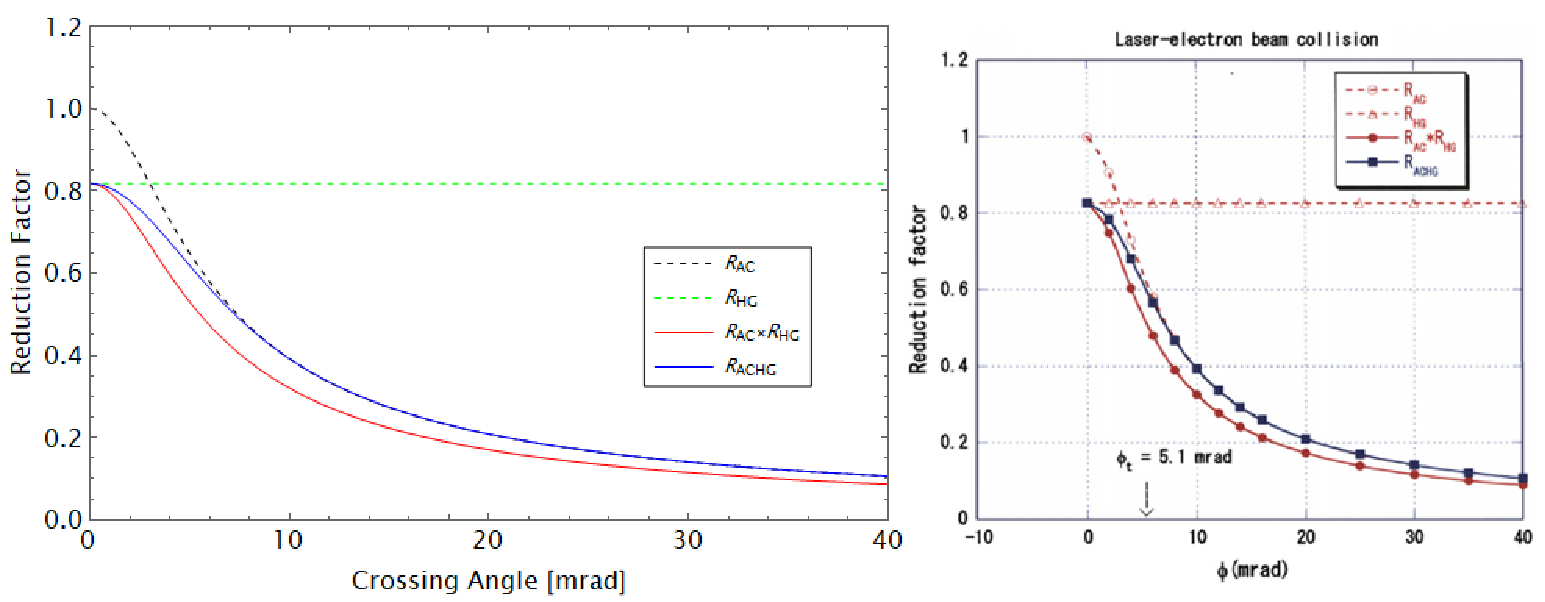
\includegraphics[width=\textwidth]{Figures/Photon_Production_by_Inverse_Compton_Scattering/miyahara_benchmarking.pdf}
\caption{Benchmarking of (Eq.~\ref{eq:miyahara_combined_reduction}) with the results of Miyahara \cite{miyahara2008luminosity}, for the Table~1 parameters and results shown in Fig.~6 of the paper. Other equations are also benchmarked such as (Eq.~\ref{eq:angular_crossing_factor}) and (Eq.~\ref{eq:furman_hourglass_reduction_analytical}). Left: Replication plot showing the angular crossing reduction $R_{AC}$ (black), hourglass reduction $R_{HG}$ (green), crudely combined reduction $R_{AC}\timesR_{HG}$ (red) and combined reduction $R_{ACHG}$ (blue). Right: Reproduction of Fig.~6 of Miyahara \cite{miyahara2008luminosity} showing the angular crossing $R_{AC}$ (red dashed circles), hourglass effect $R_{HG}$ (red dashed triangles), crude combination $R_{AC}\timesR_{HG}$ (red solid) and combined $R_{ACHG}$ (black) reduction factors.}
\label{fig:miyahara_benchmarking}
\end{figure}
Inspection of the two plots in Fig.~\ref{fig:miyahara_benchmarking} shows that they are identical with no disagreement visible. Therefore, (Eq.~\ref{eq:miyahara_combined_reduction}) is a reliable method to account for the angular crossing and hourglass effect luminosity reduction factors. 

The flux in the case of an angular collision with non-negligible divergence of electron bunches and laser pulses (hourglass effect) is given by
\begin{equation}
\mathcal{F} = \sigma R_{ACHG}\mathcal{L}_{\mathrm{HEAD-ON}}f.
\label{eq:flux_angular_crossing_hourglass}
\end{equation}
All subsequent equations, unless explicitly stated, use (Eq.~\ref{eq:flux_angular_crossing_hourglass}) to account for the geometric luminosity reduction of a ICS source.

The luminosity of this result is given by $\mathcal{L} = R_{ACHG}\mathcal{L}_{\mathrm{HEAD-ON}}$, mirroring the form of the luminosity for the isolated angular crossing and hourglass effect. Naively, one would expect the luminosity to also be appropriately modelled by $\mathcal{L} = R_{AC}R_{HG}\mathcal{L}_{\mathrm{HEAD-ON}}$, however this is incorrect as a moderate crossing angle $\phi$ will shorten the interaction time between the laser pulse and electron beam such that the interaction length is of an order at which the electron bunch and laser pulse minimally diverge and the hourglass effect is negligible. Effectively, as shown by the example calculations, a moderate crossing angle suppresses the hourglass effect.   

\section{Source Size and Divergence}
\label{sec:source_size_divergence}

The derivation of luminosity and flux in Section~\ref{sec:luminosity_and_flux} has assumed that all emission of radiation in the ICS interaction is from a point source at the centre of the interaction. However, the electron bunch--photon pulse interaction occurs in a finite spatial volume. The transverse size of this spatial volume is named the source size, the source size density of which is proportional to the transverse electron bunch electron density $n_{e}\left(x,y\right)$ and transverse laser pulse photon density $n_{L}\left(x,y\right)$ \cite{krafft2020personal}.
\begin{equation}
n_{s}\left(x,y\right) \propto n_{e}\left(x,y\right) n_{L}\left(x,y\right),
\label{eq:transverse_source_approx}    
\end{equation}
Modification of the Gaussian intensity distributions of the electron bunch (Eq.~\ref{eq:electron_gaussian_intensity_distribution}) and laser pulse (Eq.~\ref{eq:laser_gaussian_intensity_distribution}) results in the transverse densities of the photon pulse and electron bunch
\begin{align}
n_{e}\left(x,y\right) &= \frac{N_{e}}{2\pi\sigma_{e}^{2}}\exp\left(-\frac{x^{2}+y^{2}}{2\sigma_{e}^{2}}\right), 
\label{eq:transverse_electron_bunch_density}\\ 
n_{L}\left(x,y\right) &= \frac{N_{L}}{2\pi\sigma_{L}^{2}}\exp\left(-\frac{x^{2}+y^{2}}{2\sigma_{L}^{2}}\right),
\label{eq:trasverse_photon_pulse_density}
\end{align}
The transverse density of the source size (Eq.~\ref{eq:transverse_source_approx}) can be expanded through substitution of the transverse electron (Eq.~\ref{eq:transverse_electron_bunch_density}) and photon (Eq.~\ref{eq:trasverse_photon_pulse_density}) densities 
\begin{align}
n_{s}\left(x,y\right) \propto \frac{N_{e}}{2\pi\sigma_{e}^{2}}\exp\left(-\frac{x^{2}+y^{2}}{2\sigma_{e}^{2}}\right)\frac{N_{L}}{2\pi\sigma_{L}^{2}}\exp\left(-\frac{x^{2}+y^{2}}{2\sigma_{L}^{2}}\right), \nonumber \\
n_{s}\left(x,y\right) \propto \frac{N_{e}N_{L}}{2\pi\sigma_{e}^{3}\sigma_{L}^{2}}\exp\left[-\frac{\left(x^{2}+y^{2}\right)\left(\sigma_{e}^{2}+\sigma_{L}^{2}\right)}{\sigma_{e}^{2}\sigma_{L}^{2}}\right], \nonumber \\
n_{s}\left(x,y\right) \propto \frac{1}{2\pi\left(\sigma_{e}^{2}+\sigma_{L}^{2}\right)}\frac{1}{2\pi\sigma_{\gamma}^{2}}\exp\left(-\frac{x^{2}+y^{2}}{2\sigma_{\gamma}^{2}}\right),
\label{eq:expanded_transverse_source_density}    
\end{align}
where the transverse \textit{rms} source size of an inverse Compton scattering electron bunch--laser pulse interaction is consequently defined as
\begin{equation}
\sigma_{\gamma,x/y} = \frac{\sigma_{e,x/y}\sigma_{L}}{\sqrt{\sigma_{e,x/y}^{2}+\sigma_{L}^{2}}}
\label{eq:source_size}
\end{equation}
where $\sigma_{e,x/y}$ is the \textit{rms} transverse electron bunch spot size in each plane and $\sigma_{L}$ is the \textit{rms} transverse laser pulse spot size. A similar derivation to (Eq.~\ref{eq:expanded_transverse_source_density}) can be made for the longitudinal domain, therefore in the longitudinal dimension the \textit{rms} source size is given by
\begin{equation}
\sigma_{\gamma,z} = \frac{\sigma_{e,z}\left(ct_{\mathrm{pulse}}\right)}{\sqrt{\sigma_{e,z}^{2}+\left(ct_{\mathrm{pulse}}\right)^{2}}},
\label{eq:longitudinal_source_size}
\end{equation}
where $\sigma_{e,z}$ is the \textit{rms} electron bunch length and $t_{\mathrm{pulse}}$ is the \textit{rms} photon pulse duration. 

Similarly to the \textit{rms} transverse source size, the \textit{rms} source angular divergence of an ICS interaction is
\begin{equation}
\sigma_{\gamma,x/y}' = \frac{\sigma_{e,x/y}'\sigma_{L}'}{\sqrt{\sigma_{e,x/y}'^{~2}+\sigma_{L}'^{~2}}},
\label{eq:source_divergence}
\end{equation}
where $\sigma_{e,x/y}' = \sqrt{\epsilon_{x}/\beta_{x}^{*}}$ is the \textit{rms} transverse electron bunch angular divergence for a non-diffraction limited beam and $\sigma_{L} = \sqrt{\lambda/4\pi}$ is the \textit{rms} transverse laser pulse angular divergence.

A non-zero transverse source size (Eq.~\ref{eq:source_size}) suggests that photon emission from the ICS interaction can occur from any transverse position within the source size. Whilst the emission of radiation would occur mostly frequently in the centre of the bunch, due to the double Gaussian overlap, emission would be possible from the edges of the source size. A non-zero source size with possible emission from a finite transverse (Eq.~\ref{eq:source_size}) and longitudinal (Eq.~\ref{eq:longitudinal_source_size}) source size would appear to invalidate the point source approximation used in Section~\ref{sec:luminosity_and_flux}.

However, the point source approximation holds if the scattered photon distribution is sampled a large distance from the source relative to the source size i.e $\sigma_{\gamma,z} \ll d$, where $d$ is the source to collimator/detector distance. When the $\sigma_{\gamma,z} \ll d$ approximation holds this is termed far-field collimation, as this approximation is mostly utilised during discussion of collimation in ICS sources. Far-field collimation can be stated analogously in the transverse plane via $\sigma_{\gamma,x/y} \ll a$, where $a$ is the transverse size of a collimator or detector aperture downstream of the interaction. Far-field collimation is obeyed by all ICS sources designed within this work.  

\section{Spectral Density}

The spectral density of an ICS source is a measure of the energy density of the produced photon spectrum; a higher spectral density for the same scattered photon energy source means more photons are produced. The spectral density of an inverse Compton scattering source is given by
\begin{equation}
\mathcal{S} = \frac{\mathcal{F}}{E_{\gamma}^{\mathrm{MAX}}},
\label{eq:spectral_density}    
\end{equation}
where $\mathcal{F}$ is the uncollimated total flux of the ICS source given by (Eq.~\ref{eq:flux_angular_crossing_hourglass}) and $E_{\gamma}$ is the scattered photon energy (Eq.~\ref{eq:scattered_photon_energy}) at the Compton edge ($\theta = 0$). The spectral density can also be measured around the Compton edge energy for a particular bandwidth by replaceing the flux encompassed by that bandwidth, for example by replacing the raw flux $\mathcal{F}$ with the \textit{FWHM} flux in a 0.1\% bandwidth $\mathcal{F_{\mathrm{0.1\%}}}$ (Eq.~\ref{eq:flux_0.1_bandwidth}).
The spectral density around the Compton edge (Eq.~\ref{eq:compton_edge_energy}) in a 0.1\% \textit{FWHM} bandwidth is therefore
\begin{equation}
\mathcal{S}_{\mathrm{0.1\%}} = \frac{\mathcal{F_{\mathrm{0.1\%}}}}{E_{\gamma}^{\mathrm{MAX}}}.
\label{eq:spectral_density_0.1}    
\end{equation}
Framed in terms of a particular bandwidth, the spectral density becomes an important performance parameter of a narrowband ICS source. Utilising spectral density comparisons within a particular bandwidth around the Compton edge is a more appropriate comparative measure of ICS source performance as this enables a user to understand the energy density of photons available to a particular experiment from an ICS source.    

\section{Bandwidth}
\label{sec:bandwidth}

The bandwidth, the \textit{rms} energy spread of the scattered photons, is given in the recoil corrected non-linear regime ($a_{0}\ll 1$) \cite{ranjan2018simulation} by

\begin{equation}
\frac{\Delta E_{\gamma}}{E_{\gamma}} = \sqrt{\left(\frac{\sigma_{\theta}}{E_{\theta}}\right)^{2}+\left(\frac{\sigma_{e}}{E_{e}}\right)^{2}+\left(\frac{\sigma_{L}}{E_{L}}\right)^{2}+\left(\frac{\sigma_{\epsilon}}{E_{\epsilon}}\right)^{2}},
\label{eq:RMS_bandwidth}    
\end{equation}
where $\frac{\sigma_{\theta}}{E_{\theta}}$ is the collimation term, $\frac{\sigma_{e}}{E_{e}}$ is the electron beam energy spread term, $\frac{\sigma_{L}}{E_{L}}$ is the laser pulse energy spread term and $\frac{\sigma_{\epsilon}}{E_{\epsilon}}$ is the emittance terms. The terms of the bandwidth are given by
\begin{align}
\frac{\sigma_{\theta}}{E_{\theta}} &= \frac{1}{\sqrt{12}}\frac{\Psi^{2}}{1+X+\Psi^{2}/2},
\label{eq:collimation_term} \\
\frac{\sigma_{e}}{E_{e}} &= \frac{2+X}{1+X+\Psi^{2}}\frac{\Delta E_{e}}{E_{e}},
\label{eq:beam_energy_spread_term} \\
\frac{\sigma_{L}}{E_{L}} &= \frac{1+\Psi^{2}}{1+X+\Psi^{2}}\frac{\Delta E_{L}}{E_{L}},
\label{eq:laser_energy_spread_term} \\
\frac{\sigma_{\epsilon}}{E_{\epsilon}} &= \frac{\sqrt{2}\gamma^{2}}{1+X}\sqrt{\frac{\epsilon_{x}^{2}}{\beta_{x}^{*2}}+\frac{\epsilon_{y}^{2}}{\beta_{y}^{*2}}}
\label{eq:emittance_term}
\end{align}
where $\Psi = \gamma\theta$ is the acceptance angle, $\epsilon_{x/y}$ is the emittance in the $x$ or $y$ direction, $\beta_{x/y}^{*}$ are the $\beta$ functions at the IP in both directions, $\Delta E_{e}/E_{e}$ is the \textit{rms} relative energy spread of the electron bunch and $\Delta E_{L}/E_{L}$ is the \textit{rms} spectral bandwidth of the laser pulse. The \textit{rms} bandwidth can trivially be converted into the full width half maximum (FWHM) bandwidth 
\begin{equation}
\left(\frac{\Delta E_{\gamma}}{E_{\gamma}}\right)_{\mathrm{FWHM}} = 2\sqrt{2\ln{2}}\left(\frac{\Delta E_{\gamma}}{E_{\gamma}}\right)_{rms}.
\label{eq:FWHM_bandwidth}
\end{equation}

Other formulations of the \textit{rms} bandwidth exist such as the formulation used by Akagi et al \cite{akagi2016narrow} derived by Petrillo et al \cite{petrillo2012photon}, where notation has been standardised to that used in this text 
\begin{equation}
\frac{\Delta E_{\gamma}}{E_{\gamma}} = \sqrt{\Psi^{4}+4\left(\frac{\Delta E_{e}}{E_{e}}\right)^{2}+\left(\frac{\epsilon_{n}}{\sigma_{e}}\right)^{4}+\left(\frac{\Delta\nu}{\nu}\right)^{2}+\left(\frac{M^{2}\lambda}{4\pi\sigma_{L}}\right)^{4}},
\label{eq:akagi_bandwidth}    
\end{equation}
where $\epsilon_{n}=\epsilon_{n,x}=\epsilon_{n,y}$ is the round beam normalised transverse emittance, $\sigma_{e}$ is the round beam electron bunch spot size, $\Delta\nu/\nu$ is the spectral bandwidth of the laser pulse defined in terms of the laser pulse frequency $\nu$ and $M^{2}$ is the quality factor of the laser pulse ($M^{2} = 1$ for a perfectly Gaussian laser pulse). In comparison to (Eq.~\ref{eq:RMS_bandwidth}), the formulation used by Akagi et al \cite{akagi2016narrow} is very simplistic in the treatment of the emittance term $\left(\epsilon_{n}/\sigma_{e}\right)^{4}$, which takes into account the only the round beam divergence, and the collimation term $\Psi^{4}$ which is only the acceptance angle. The Petrillo et al bandwidth is therefore only valid in the round beam case ($\epsilon_{n,x} = \epsilon_{n,y} = \epsilon_{n}$). Recoil of the electron bunch has also not been accounted for in any term so the Petrillo et al bandwidth is only relevant in the Thomson regime ($X \ll 1$) and angular variation is only accounted for in the collimation term not, as in (Eq.~\ref{eq:RMS_bandwidth}), for the electron bunch $4\left(\Delta E_{e}/E_{e}\right)^{2}$ and laser pulse $\left(\Delta\nu/\nu\right)^{2}$ energy spread terms. Unlike in (Eq.~\ref{eq:RMS_bandwidth}) a laser pulse quality term $\left(M^{2}\lambda/4\pi\sigma_{L}\right)^{4}$ is imposed however this term is generally negligible because miniscule foci of the laser pulses required to make this term non-negligible are beyond limits of laser science. For example, for a Gaussian ($M^{2}=1$) Nd:YAG laser ($\lambda = 1064$~\si{\nano\meter}) pulse focused to a typical small laser pulse \textit{rms} spot size of 30~\si{\micro\meter} this term makes a $7.97\times 10^{-6}$ contribution to the \textit{rms} bandwidth hence it is neglected by Ranjan et al \cite{ranjan2018simulation} in the selected \textit{rms} bandwidth (Eq.~\ref{eq:RMS_bandwidth}).   

Another possible formulation has been suggested by Curatolo et al \cite{curatolo2017analytical}, which updates (Eq.~\ref{eq:akagi_bandwidth})
\begin{multline}
\frac{\Delta E_{\gamma}}{E_{\gamma}} = \left\{\left[\frac{\Psi^{2}}{\sqrt{12}\left(1+\Psi^{2}\right)}+\frac{\bar{P}^{2}}{1+\sqrt{12}\bar{P}^{2}}\right]^{2}+\left[\left(\frac{2+X}{1+X}\right)\frac{\Delta E_{e}}{E_{e}}\right]^{2}+\left(\frac{1}{1+X}\frac{\Delta E_{L}}{E_{L}}\right)^{2} \right.\\\left. +\left(\frac{M^{2}\lambda}{4\pi\sigma_{L}}\right)^{4}+\left(\frac{a_{0}^{2}/3}{1+a_{0}^{2}/2}\right)^{2}\right\}^{1/2}
\label{eq:curatolo_bandwidth}    
\end{multline}
where 
\begin{equation}
\bar{P} = \frac{\sqrt{2}\epsilon_{n}}{\sigma_{e}\sqrt{1+X}},
\label{eq:curatolo_p_bar}    
\end{equation}
is the \textit{rms} normalised transverse momentum of the electron bunch. The bandwidth formulation by Curatolo et al assumes a round transverse profile of the electron bunch as in (Eq.~\ref{eq:akagi_bandwidth}), and also includes an identical negligible beam quality term. Recoil correction is included in (Eq.~\ref{eq:curatolo_bandwidth}) but angular variation is only included in the collimation term, as the acceptance angle is present in no other term. A non-linear ponderomotive broadening term $\left(\frac{a_{0}^{2}/3}{1+a_{0}^{2}/2}\right)^{2}$ is introduced in (Eq.~\ref{eq:curatolo_bandwidth}), which is advantageous over the bandwidth by Ranjan et al \cite{ranjan2018simulation}. The bandwidth by Curatolo et al \cite{curatolo2017analytical} also includes covariance of the emittance and collimation terms for predicting the bandwidth of skewed non-Gaussian spectra \cite{ranjan2018simulation}. However skewed non-Gaussian spectra effects are also accounted for by Ranjan et al in an equation of the form
\begin{equation}
\frac{\Delta E_{\gamma}}{E_{\gamma}} = \sqrt{\left[\left(\frac{\sigma_{\theta}}{E_{\theta}}\right)+\left(\frac{\sigma_{\epsilon}}{E_{\epsilon}}\right)\right]^{2}+\left(\frac{\sigma_{e}}{E_{e}}\right)^{2}+\left(\frac{\sigma_{L}}{E_{L}}\right)^{2}},
\label{eq:covariant_RMS_bandwidth}    
\end{equation}
where the emittance and collimation terms are covariant. The covariant form is not utilised in this work as there is a focus on Gaussian electron bunches and laser pulses, and (Eq.~\ref{eq:RMS_bandwidth}) produces the same result as (Eq.~\ref{eq:covariant_RMS_bandwidth}) for Gaussian ICS spectra. All optimisation methods in Chapter~\ref{Optimisation_and_Characterisation_of_Inverse_Compton Scattering_Spectra} can be utilised with the covariant form, however as standard (Eq.~\ref{eq:RMS_bandwidth}) is used. 

Therefore, (Eq.~\ref{eq:RMS_bandwidth}) was selected as this is both recoil corrected and accounts for angular variation in each bandwidth term, it is valid in the linear ($a_{0}\ll 1$) region of interest and most importantly, properly accounts for non-round electron bunch transverse profiles by allowing for asymmetric emittance. The beam quality term is neglected which improves calculation speed. As shown in Fig.~1 of Ranjan et al \cite{ranjan2018simulation} (reproduced in Fig.~\ref{}), there is also an apparent discrepancy in how the collimation angle, via the acceptance angle, is accounted for in the Curatolo et al equation (Eq.~\ref{eq:curatolo_bandwidth}). Whilst the semi-analytical spectrum code \textsc{ICCS3D} \cite{krafft2016laser,ranjan2018simulation} (explained further in Chapter~\ref{Optimisation_and_Characterisation_of_Inverse_Compton Scattering_Spectra}) and (Eq.~\ref{eq:RMS_bandwidth}) show good agreement, (Eq.~\ref{eq:curatolo_bandwidth}) shows a systematic variance from the simulations. The combination of these factors provided the motivation for selecting (Eq.~\ref{eq:RMS_bandwidth}) as the \textit{rms} bandwidth formulation.
\begin{figure}[!h]
\centering
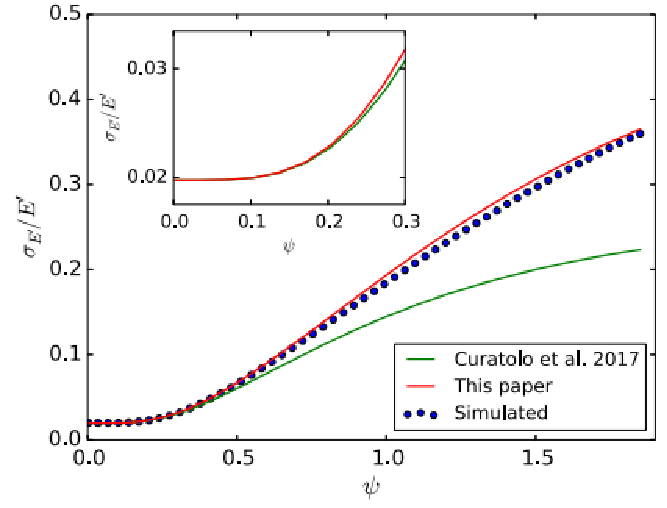
\includegraphics[width=0.7\textwidth]{Figures/Photon_Production_by_Inverse_Compton_Scattering/ranjan_curatolo_disagreement.pdf}
\caption{Reproduction of Fig.~1 of Ranjan et al \cite{ranjan2018simulation}. \textit{Rms} bandwidth of an ICS source as a function of acceptance angle, using the case $A_{a}$ parameters by Ranjan et al \cite{ranjan2018simulation}, for (Eq.~\ref{eq:RMS_bandwidth}) (red, Ranjan et al \cite{ranjan2018simulation}) and (Eq.~\ref{eq:curatolo_bandwidth}) (green, Curatolo et al \cite{curatolo2017analytical}) and the \textsc{ICCS3D} simulated spectrum bandwidths (black points, Ranjan et al \cite{ranjan2018simulation}). }
\label{fig:curatolo_ranjan_disagreement}
\end{figure}

However, there are some downsides to the Ranjan et al formulation (Eq.~\ref{eq:RMS_bandwidth}), as this is incapable of calculating the bandwidth for a non-linear ($a_{0}\sim 1$) ICS source. Circular collimation is also assumed implicitly by the inclusion of a single acceptance angle term $\Psi$, as in the rectangular collimator case the maximum collimation angle would vary in the $x$ and $y$ plane. The bandwidth in (Eq.~\ref{eq:RMS_bandwidth}) has been extended to rectangular collimation by Hajima \cite{hajima2021bandwidth}. 

\section{Peak and Average Brilliance}
\label{sec:peak_average_brilliance}

Brilliance, also interchangeably termed brightness, is a quantity originally used to quantify the 6D phase space density of particle beams \cite{courant1958theory}. Here brilliance has been selected to describe photon beams and brightness to describe the similar concept in electron beams. This concept was adopted to characterize radiation beams produced from accelerator driven light sources, such as bending magnet or wiggler synchrotron radiation sources and undulators \cite{kim1989characteristics}, where the brilliance is defined as the flux into a cone of particular spectral bandwidth (usually 0.1\%) per unit phase space area. The brilliance performance parameter is readily applied to free electron lasers \cite{krinsky1983undulators,kim1987brightness} and has been extended to ICS sources \cite{hartemann2005high,krafft2010compton}.  

Average brilliance is time averaged, summing the contribution of all electron bunch--laser pulse interactions of the source, thereby accounting for the repetition rate of the interactions. Whereas, peak brilliance is calculated for a single bunch--pulse interaction subject to the interaction time. Experimentally, both peak and average brilliance have advantages, peak brilliance is useful for analysing fast processes beyond the repetition rate of ICS sources or taking destructive measurements -- similar to the utility of x-ray FELs -- whereas average brilliance excels in improving data acquisition rates in processes with small cross sections, such as nuclear resonance fluorescence studies \cite{angell2015demonstration}. Linac driven ICS sources typically are designed to be single-shot, high peak brilliance sources whereas storage ring and recirculated electron beam based ICS sources take advantage of high repetition rates to be high average brilliance sources. Theoretically, ERL's with linac quality recirculated electron beams could dually provide high peak and average brilliance.   

Often ICS sources are viewed as analagous to undulator radiation, a 'laser undulator' system. Hence, the average brilliance of an ICS source is adapted from that of an undulator. The average brilliance of an undulator source assuming a Gaussian electron bunch and planar undulator field \cite{chao2013handbook} is given by 
\begin{equation}
\mathcal{B}_{U} = \frac{\Phi_{n}}{4\pi^{2}\Sigma_{x}\Sigma_{y}\Sigma_{x}'\Sigma_{y}'}
\label{eq:undulator_brightness}    
\end{equation}
where $\Phi_{n}$ is the total spectral flux of the $n$th undulator harmonic generate into a central cone of 0.1\% spectral bandwidth, $\Sigma_{x/y} = \sqrt{\sigma_{x/y}^{2}+\sigma_{R}^{2}}$ are the source sizes of the interaction in each plane with $\sigma_{x/y}$ the \textit{rms} source size of the electron beam and $\sigma_{R}$ the diffraction limited source size of a single electron emission \cite{kim1987brightness}, and $\Sigma_{x/y}' = \sqrt{\sigma_{x}'^{2}+\sigma_{R}'^{2}}$ the source size divergences with $\sigma_{x}'$ the \textit{rms} divergence of the electron beam and $\sigma_{R}'$ the \textit{rms} angular divergence of the single electron emission \cite{krinsky1983undulators}. 

The average brilliance for an inverse Compton scattering source is defined as the average flux per unit phase space area of the interaction per 0.1\% \textit{rms} bandwidth. The ICS average brilliance, is modified from the undulator brilliance (Eq.~\ref{eq:undulator_brightness}) through replacement of the single electron emission field for the electric field of a Gaussian laser pulse \cite{krafft2010compton,deitrick2018high}
\begin{equation}
\mathcal{B}_{\mathrm{avg}} = \frac{\mathcal{F}_{0.1\%}}{4\pi^{2}\sigma_{\gamma,x}\sigma_{\gamma,x}'\sigma_{\gamma,y}\sigma_{\gamma,y}'},
\label{eq:average_brilliance}
\end{equation}
where $\mathcal{F}_{0.1\%}$ is the flux in a 0.1\% FWHM bandwidth (Eq.~\ref{eq:flux_0.1_bandwidth}) using the modified form of the flux for geometric luminosity reduction (Eq.~\ref{eq:flux_angular_crossing_hourglass}), $\sigma_{\gamma,x/y}$ are the source sizes in each plane (Eq.~\ref{eq:source_size}) and $\sigma_{\gamma,x/y}'$ are the source angular divergences (Eq.~\ref{eq:source_divergence}) in each plane. Assuming a non-diffraction limited electron bunch and that $\sigma_{e,x/y}' > \sigma_{L}'$, the brilliance can be roughly calculated as
\begin{equation}
\mathcal{B}_{\mathrm{avg}} = \frac{\mathcal{F}_{0.1\%}}{4\pi^{2}\sigma_{\gamma,x}\sqrt{\epsilon_{x}/\beta_{x}^{*}}\sigma_{\gamma,y}\sqrt{\epsilon_{y}\beta_{y}^{*}}},
\label{eq:average_brilliance_nondiffraction}    
\end{equation}
simplifying (Eq.~\ref{eq:average_brilliance}) further, by conceding that for a compact ICS source the electron bunch transverse profile size typically dominates the laser spot size ($\sigma_{e,x/y}\gg\sigma_{L}$) i.e $\sigma_{\gamma,x/y} \approx \sqrt{\epsilon_{x/y}\beta_{x/y}^{*}}$, the average brilliance becomes
\begin{equation}
\mathcal{B}_{\mathrm{avg}} \approx \frac{\gamma^{2}\mathcal{F}_{0.1\%}}{4\pi^{2}\epsilon_{n,x}\epsilon_{n,y}},
\label{eq:average_brilliance_compact}    
\end{equation}
therefore the average brilliance is approximately proportional to the Lorentz factor squared ($\mathcal{B}\propto 1/\gamma^{2}$). 

However, assuming $\sigma_{L}<\sigma_{e}$ is often incorrect for the source designs presented in this report and in Chapter~\ref{Optimisation_and_Characterisation_of_Inverse_Compton Scattering_Spectra} in Section~\ref{sec:transverse_profile_matching} a case is made for sources to obey $\sigma_{L}>\sigma_{e}$, therefore (Eq.~\ref{eq:average_brilliance_compact}) is not selected. The angular divergence of the electron bunch is also not typically larger that the angular divergence of the laser pulse in a narrowband ICS source. For example, using the derivations of Section~\ref{sec:source_size_divergence}, a Nd:YAG laser ($\lambda = 1064$~\si{\nano\meter}) interacting with a $E_{e} = 500$~\si{\mega\electronvolt} kinetic energy electron bunch with a 0.5~\si{\mill\meter}--\si{\milli\radian} normalised emittance in each plane at a focus of $\sigma_{e} = 10$~\si{\centi\meter} in each plane has an electron bunch angular divergence of $\sigma_{e}' = 7.14\times10^{-5}$ and a laser pulse angular divergence of $\sigma_{L}' = 2.91\times 10^{-4}$. Clearly, the effect of the laser pulse angular divergence in (Eq.~\ref{eq:average_brilliance}) can not be neglected in all cases, and is highly sensitive to electron bunch focusing parameters. Subsequently, (Eq.~\ref{eq:average_brilliance}) is favoured over the case in which the laser pulse angular divergence is neglected (Eq.~\ref{eq:average_brilliance_nondiffraction}).  

The peak brilliance, as derived by Hartemann and Brown \cite{hartemann2005high}, is given by
\begin{multline}
\mathcal{B}_{\mathrm{pk}} = \frac{4\times 10^{-15}}{\pi^{2}}\frac{\gamma}{\epsilon_{n}^{2}}\frac{N_{e}N_{L}}{t_{\mathrm{bunch}}}\frac{r_{e}^{2}}{4\sigma_{L}^{2}}\exp\left\{\frac{\chi-1}{2\chi\Delta u_{\perp}^{2}}\left[2+\frac{\delta\omega^{2}+\delta\gamma^{2}\chi^{2}}{2\chi\left(\chi-1\right)\Deltau_{\perp}^{2}}\right]\right\} \\ \left[1-\Phi\left\{\frac{\chi-1}{\sqrt{\delta\omega^{2}+\delta\gamma^{2}\chi^{2}}}\left[1+\frac{\delta\omega^{2}+\delta\gamma^{2}\chi^{2}}{2\cji\left(\chi-1\right)\Delta u_{\perp}^{2}}\right]\right\}\right]\left\{\frac{\eta e^{1/\mu^{2}\left[\Phi\left(1/\eta\right)-1\right]-\mu e^{1/\eta^{2}}\left[\Phi\left(1/\mu\right)-1\right]}}{\mu^{2}-\eta^{2}}\right\},
\label{eq:hartemann_peak_brilliance}    
\end{multline}
where $\chi = E_{\gamma}/4\gamma^{2}E_{L}$ is the normalised Doppler up-shifted frequency, $\Delta u_{\perp} \approx \epsilon_{n}/\sigma_{e}$ is the approximated transverse spread in electron velocity,  $\delta\omega = 2\Delta E_{L}/E_{L}$, the relative spectral bandwidth of the laser pulse, $\delta\gamma = \Delta E_{e}/E_{e}$, the relative electron bunch energy spread, $\Phi\left(x\right)$ is the standard Gaussian error function (Eq.~\ref{eq:error_function}), $\eta = ct_{\mathrm{pulse}}/2\sqrt{2}\beta^{*}$ is the normalised inverse $\beta$-function at the IP and $\mu = ct_{\mathrm{pulse}}/2\sqrt{2}z_{R}$ is the normalised Rayleigh length. As the brilliance is quoted in \si{\milli\radian}$^{2}$--\si{\milli\meter}$^{2}$ per 0.1\% bandwidth, a factor $10^{-15}$ is present in (Eq.~\ref{eq:hartemann_peak_brilliance}) to account for the SI unit conversion and bandwidth selection; a $10^{-6}$ factor originates from \si{\milli\radian} to \si{rad} conversion, similarly a $10^{-6}$ factor occurs for the \si{\milli\meter} to \si{\meter} conversion plus a factor of $10^{-3}$ is introduced due to the per mille bandwidth (0.1\%) which sums to produce the $10^{-15}$ factor.

The analytical peak brillance calculation by Hartemann and Brown \cite{hartemann2005high} is advantageous because the energy spread of the electron bunch and spectral bandwidth of the laser pulse are accounted for in the calculation. There is also an attempt to account for the geometric luminosity reduction via an overlap function in the final term of (Eq.~\ref{eq:hartemann_peak_brilliance}), which is essentially accounting for the hourglass effect \cite{furman1991hourglass} (Eq.~\ref{eq:furman_hourglass_reduction}), though the functional form is only valid for the round beam case ($\epsilon_{n,x} = \epsilon_{n,y} = \epsilon_{n}$) and doesn't account for an angular crossing either ($\phi\neq0$), unlike the Miyahara luminosity reduction \cite{miyahara2008luminosity} (Eq.~\ref{eq:miyahara_combined_reduction}) which is more general. The Hartemann and Brown equation (Eq.~\ref{eq:hartemann_peak_brilliance}) is therefore only valid in the head-on ($\phi=0$) case and for a round electron bunch transverse profile. Electron recoil arising from scattering with high kinetic energy electron bunches is also not accounted for within this model.

The peak brilliance can also be constructed by modifying the average brilliance (Eq.~\ref{eq:average_brilliance}) via time averaging a single interaction, as is pursued in Curatolo et al \cite{curatolo2017analytical}. The peak bandwidth, based on the average brilliance formulation (Eq.~\ref{eq:average_brilliance}) by Deitrick et al \cite{deitrick2018high}, becomes
\begin{equation}
\mathcal{B}_{\mathrm{pk}} = \frac{c}{2\sqrt{2\ln2}\sigma_{\gamma,z}}\frac{N_{0.1\%}}{4\pi^{2}\sigma_{\gamma,x}\sigma_{\gamma,x}'\sigma_{\gamma,y}\sigma_{\gamma,y}'},
\label{eq:peak_brilliance}    
\end{equation}
where time averaging is introduced via the interaction time $\sigma_{\gamma,z}/c$ with $\sigma_{\gamma,z}$ the \textit{rms} longitudinal source size (Eq.~\ref{eq:longitudinal_source_size}) -- which is converted to FWHM -- and the no. photons scattered into a 0.1\% FWHM bandwidth given by $N_{0.1\%} = 3/2\times 10^{-3}\mathcal{F}$ with $\mathcal{F}$ the flux corrected for geometric luminosity reduction (Eq.~\ref{eq:flux_angular_crossing_hourglass}). The peak brilliance formula in (Eq.~\ref{eq:peak_brilliance}) is recoil corrected, applicable to a non-round transverse profile and to an angular crossing via the gemoetrical luminosity reduction (Eq.~\ref{eq:miyahara_combined_reduction}). However, unlike (Eq.~\ref{eq:hartemann_peak_brilliance}), the energy spread of the electron bunch and the spectral bandwidth of the laser pulse are neglected. 

Comparison of (Eq.~\ref{eq:hartemann_peak_brilliance}) and (Eq.~\ref{eq:peak_brilliance}) has shown that the Hartemann and Brown peak brilliance is adequate for cases where interactions are head-on and recoil is small ($X \ll 1$) but unsatisfactory for non-round transverse electron bunch profiles or interactions which occur at an angle. Whilst the relative electron bunch energy spread is typically on the scale of $10^{-3}$--$10^{-4}$ (0.1--0.01\%), for example in cERL \cite{akagi2016narrow} ($\Delta E_{e}/E_{e}$ = 0.1\%) and in the MAX-III storage ring \cite{sjostrom2009max} ($\Delta E_{e}/E_{e}$ = 0.061\%), and the laser pulse is typically on the scale of $10^{-2}$--$10^{-5}$ (1--0.001\%), for example in the cERL ICS experiment ($\Delta E_{L}/E_{L}$ = 0.006\%) \cite{akagi2016narrow} and for high-powered Ti:Sa laser systems ($\Delta E_{L}/E_{L}$ = 1.19\%) \cite{liu2021review}, this is a much smaller effects than an angular crossing, as evident from (Eq.~\ref{eq:angular_crossing_factor}) in Section~\ref{sec:geometric_luminosity_reduction}, where a 5\si{\degree} crossing angle results in a 78\% luminosity reduction. Therefore, (Eq.~\ref{eq:peak_brilliance}) should be favoured in angular crossing ($\phi\neq 0$) situations unless the energy spread and spectral bandwidth are particularly large contrary to most ICS source designs. A case of asymmetric emittance can also not be handled by (Eq.~\ref{eq:hartemann_peak_brilliance}), therefore these must be calculated by (Eq.~\ref{eq:peak_brilliance}). Throughout this work the peak brillance calculation used, either (Eq.~\ref{eq:hartemann_peak_brilliance}) or (Eq.~\ref{eq:peak_brilliance}), will be noted in the footnotes of the relevant table.  

\end{document}